\documentclass[11pt]{article}
\input{glyphtounicode-cmr}
\pdfgentounicode=1
\usepackage[T1]{fontenc}
\usepackage[utf8]{inputenc}
\usepackage{lmodern}
\usepackage[margin=1.05in]{geometry}
\usepackage{amsmath,amssymb,amsthm,mathtools}
\usepackage{microtype,enumitem,booktabs,needspace}
\usepackage{tikz}
\usetikzlibrary{arrows.meta,positioning,calc}
\usepackage{xcolor}
\usepackage[hyphens]{url}
\usepackage[colorlinks=true,linkcolor=blue!45!black,citecolor=blue!45!black,urlcolor=blue!45!black]{hyperref}
\ifdefined\pdfinfoomitdate\pdfinfoomitdate=1\fi
\ifdefined\pdftrailerid\pdftrailerid{}\fi
\ifdefined\pdfsuppressptexinfo\pdfsuppressptexinfo=15\fi
\newtheorem{theorem}{Theorem}[section]
\newtheorem{lemma}[theorem]{Lemma}
\newtheorem{proposition}[theorem]{Proposition}
\newtheorem{corollary}[theorem]{Corollary}
\theoremstyle{definition}
\newtheorem{definition}[theorem]{Definition}
\theoremstyle{remark}
\newtheorem{remark}[theorem]{Remark}
\newcommand{\ED}{\operatorname{ED}}
\newcommand{\LCS}{\operatorname{LCS}}
\newcommand{\E}{\mathbb E}
\newcommand{\TV}{\operatorname{TV}}
\newcommand{\eps}{\varepsilon}
\DeclareMathOperator{\supp}{supp}
\setlength{\emergencystretch}{2em}
\allowdisplaybreaks[1]
\title{Finite-Circle Obstructions, Binary Codes, and\\
Histogram Embeddings for Edit Distance}
\author{OpenAI}
\date{September 27, 2026}
\hypersetup{pdftitle={Finite-Circle Obstructions, Binary Codes, and Histogram Embeddings for Edit Distance},pdfauthor={OpenAI}}
\begin{document}
\maketitle
\begin{abstract}
We give two finite-circle constructions of binary strings whose least
$\ell_1$ distortion is
$\exp(\Omega(\sqrt{\log d\,\log\log d}))$, where $d$ bounds their length.
Both constructions supply words of one common length for every sufficiently
large cap. Two direct binary coding arguments transfer the constructions
with absolute distortion and logarithmic block width. We also develop the
overlapping-substring method of Ostrovsky and Rabani into a complete finite
histogram embedding at the same exponential scale, uniformly over all
finite alphabets and all words of length at most $d$, including the empty word.
\end{abstract}

\section{Introduction}\label{sec:introduction}

An insertion or deletion changes the positions of every later symbol.
Yet cyclically shifting a nonempty word by one position costs at most two edits: delete its first
symbol and insert it at the end. We use the difference between the length of
a word and the cost of translating it to study how faithfully edit distance
can be represented in $\ell_1$.

\paragraph{The metric and the question.}
For finite words $x,y$, let $\ED(x,y)$ be the least number of single-symbol
insertions, deletions, and substitutions taking $x$ to $y$, with each
operation costing one. If $\Sigma$ is a finite alphabet with at least two
symbols and $d\geq1$ is an
integer, let $\Sigma^{\leq d}$ contain all words of length at most $d$,
including the empty word. This cap restricts only the endpoints of a
comparison; intermediate words in an edit script are unrestricted.
For an injective map $f:\Sigma^{\leq d}\to\ell_1$, its distortion is
\[
 \operatorname{dist}(f)=
 \left(\max_{x\ne y}\frac{\|f(x)-f(y)\|_1}{\ED(x,y)}\right)
 \left(\max_{x\ne y}\frac{\ED(x,y)}{\|f(x)-f(y)\|_1}\right),
 \qquad E_\Sigma(d)=\inf_f\operatorname{dist}(f).
\]
Here $\ell_1$ is the real space of absolutely summable sequences. There is
no restriction on target dimension or on how the map is computed. The
question asks for one map that represents every pair in the domain.

\begin{theorem}\label{thm:main}
There are absolute constants $c,C>0$ and an integer $d_0$ such that, for
every integer $d\geq d_0$ and every finite alphabet $\Sigma$ with
$|\Sigma|\geq2$,
\begin{equation}\label{eq:main}
 \exp\!\bigl(c\sqrt{\log d\,\log\log d}\bigr)
 \leq E_\Sigma(d)\leq
 \exp\!\bigl(C\sqrt{\log d\,\log\log d}\bigr).
\end{equation}
Each of our two lower constructions supplies a binary subset whose words
have one common length at most $d$ and whose least $\ell_1$ distortion
satisfies the lower bound. The upper bound is realized by a deterministic
finite-dimensional map.
\end{theorem}

All logarithms are natural unless a base is displayed. The constants are
independent of the finite alphabet, including alphabets whose size grows
with $d$. Thus the same estimates hold for
$\sup_{2\leq|\Sigma|<\infty}E_\Sigma(d)$. Equation~\eqref{eq:main}
determines the order of $\log E_\Sigma(d)$; the constants in its two
exponents need not agree.

\paragraph{Earlier bounds and the role of alignment.}
The single-symbol error model has its roots in Levenshtein's work on
insertion and deletion codes \cite{Levenshtein1966}. Wagner and Fischer's
increasing traces describe the alignments available to two words
\cite{WagnerFischer1974}. In particular, if $\LCS(x,y)$ denotes the longest
common subsequence length, the insertion--deletion distance is
\[
 \Delta(x,y)=|x|+|y|-2\LCS(x,y),\qquad
 \ED(x,y)\leq\Delta(x,y)\leq2\ED(x,y).
\]
A lower bound must therefore control arbitrary increasing matchings, even
when they cross many of the boundaries used to construct the words.

Ostrovsky and Rabani obtained the upper scale in Theorem~\ref{thm:main} for
fixed-length binary edit distance by recursively comparing multisets of
overlapping substrings \cite{OstrovskyRabani2007}. They also noted extensions
to larger alphabets and varying lengths. Section~\ref{upper:section} gives
a complete finite histogram construction with alphabet-independent constants
and all shorter words included. It can be read on its own.

For lower bounds, Andoni, Deza, Gupta, Indyk, and Raskhodnikova found binary
sets whose $L_1$ distortion approaches $3/2$
\cite{AndoniDezaGuptaIndykRaskhodnikova2003}. Their construction uses several
nearby word lengths. Khot and Naor obtained a
$(\log d)^{1/2-o(1)}$ bound using Fourier analysis of cuts and noisy shifts
\cite{KhotNaor2006}; their insertion--deletion convention transfers to ours
within a factor of two. Krauthgamer and Rabani strengthened the bound to
$\Omega(\log d)$ on binary words of length $d$
\cite[Theorem~1.3]{KrauthgamerRabani2009}. Our constructions use the same
broad cut and Fourier viewpoint, but impose translation constraints through
distinct prime periods. Those constraints force large total leaf frequency
and yield the exponent in~\eqref{eq:main}. The resulting lower bound grows
faster than every fixed power of $\log d$, while remaining $d^{o(1)}$.
Thus it reaches the scale of the Ostrovsky--Rabani upper bound after taking
logarithms.

\paragraph{The lower constructions.}
A phase is a point of the circle $\mathbb R/\mathbb Z$. We work on a finite
equally spaced grid containing the half-turn $1/2$. A state assigns one grid
phase to each leaf of a finite rooted tree. At a leaf, a binary pattern
records a translated half-circle on that grid. At an internal node, a row
lists the child words, each with its own tag; a long word repeats rows at
translated phases.

Both constructions compare three kinds of phase change. Translations in a
specified subgroup move the row lists at low edit cost. Moving just one
leaf changes only the fraction of the word occupied by that leaf, with
edit cost at most twice the occupied length times the phase displacement.
A simultaneous half-turn at every leaf must have a large edit cost. This last
assertion requires control of arbitrary alignments: a matching may cross
many of the rows used to define the words.

The row tags provide that control. A source row whose matches stay in one
target row inherits the child separation. If its matches enter several
target rows, they leave a long unmatched target interval. The intervals
charged by distinct source rows are disjoint. Lemma~\ref{pre:tagged-rows}
turns this observation into the separation estimate used by both
constructions.

To compare these edit costs with an arbitrary $\ell_1$ image, we express
its distances on the finite phase space as nonnegative sums of cut distances
and then use finite Fourier expansion. A character has one integer frequency
at each leaf. Averaging over the cheap subgroup controls the total Fourier
weight of characters nonconstant on it. Among the remaining characters,
one that detects the half-turn must have large total absolute leaf
frequency: if that total were small, the prime constraints would force
nonzero frequency sums to branch through too many leaves. Weighted
single-leaf shifts control the Fourier mass carried by these large
frequencies.
The common analytic step is Lemma~\ref{pre:weighted-circle}; each construction proves
its own arithmetic branching bound.

The two prime patterns also give different proofs of half-turn separation.
The first construction groups children by primes and includes every residue
of each prime. Its separation proof follows a nonzero phase down the tree
while keeping track of the loss at each level. The complete residue lists
allow the descent to restart at the reciprocal of a single prime; these
resets keep the denominator factors acquired at other steps from
accumulating without control. The accumulated losses and the final phase's
distance from zero give a quantitative lower bound for the half-turn.
Section~\ref{sec:masks} constructs the words and carries out this descent.

The second construction uses one child per prime, with that prime's
translation acting on every child except its own. Two child phases of small
cost would have a small difference involving at most two fresh prime
denominators. The induction rules out every nonzero such difference, forcing
most translation coordinates to vanish. Section~\ref{sec:excluded} develops
this separate argument.

\paragraph{Binary transfer and the upper construction.}
The tags initially require a larger alphabet. Section~\ref{p2:sec:binary-coding}
gives two direct binary substitutions of width $O(\log(2A))$ for an alphabet
of size $A$. Each has absolute distortion on all equal-length words,
simultaneously for every common length. One proof separates intervals of
differently labelled codewords and uses a common offset to recover a letter
matching. The other controls shifted self-overlaps and finds anchors at equal
relative indices. The lower constructions use these bounds only at equal lengths.

The same existence order follows from the alphabet reduction of
Bhattacharya, Dey, Goldenberg, and Kouck\'y \cite[Theorem~1.1 and Section~3.2.1 of the full version]{BhattacharyaDeyGoldenbergKoucky2024}.
Their stated theorem approximately preserves normalized insertion--deletion
distance, with each distance divided by the sum of the lengths of its two
arguments. The block substitution in its proof has logarithmic width for a
fixed target alphabet. Composing that substitution
with a fixed-width binary delimiter gives the claimed binary width and
distortion, as we explain in Section~\ref{p2:sec:binary-coding}. Our direct proofs expose two different
local matching conditions. Long-interval separation is already present
in Schulman and Zuckerman's inner code \cite[Section~II-C]{SchulmanZuckerman1999},
and self-matching control is a central feature of synchronization strings
\cite{HaeuplerShahrasbi2017}.

For either lower route, depth $h$ gives logarithmic distortion of order
$h\log h$ at lengths whose logarithms are $O(h^2\log h)$. The direct
parameter choice in Section~\ref{sec:assembly} supplies every sufficiently
large cap. Finally, Section~\ref{upper:section} develops the independent
upper construction: divide words into blocks, list overlapping windows,
partition their shorter-word images using cuts, and record the resulting
histograms. After the power-length proof, a map at actual window lengths
admits two expansion estimates, one from an arbitrary longest common
subsequence and one from moves. A final variant uses total variation.

Theorem~\ref{thm:uniform-upper} supplies the upper embedding stated as
Theorem~6.1 of the companion tree constructions \cite{OpenAITree2026},
which is combined with their lower bounds in Corollary~6.2. Their lower
proofs are independent of the present constructions.
A shorter companion proof \cite{OpenAIMain2026} uses marked rows and a
prime-product displacement inequality, with no lower-proof dependence on
the circle constructions.

\section{Alignments and tagged rows}\label{sec:preliminaries}

We first relate edit distance to increasing subsequence matchings, then
transfer a separation estimate for tagged child words to an estimate for
rows under arbitrary alignments. This is the only general tool needed
before constructing the circle words.

\subsection{Subsequence deficit and tagged rows}
A common subsequence is a collection of equal-symbol pairs whose position
indices increase strictly on both sides. Write $\LCS(x,y)$ for its maximum
size. For equal-length words of length $n$, put
\[
 r_n(x,y)=n-\LCS(x,y).
\]
This is the number of unmatched positions on either side of a longest
common subsequence. For arbitrary lengths put
$q(x,y)=\max(|x|,|y|)-\LCS(x,y)$.

\begin{lemma}[Metric comparisons]\label{pre:metric}
For all finite words $x,y$,
\[
 q(x,y)\leq\ED(x,y)\leq2q(x,y),\qquad
 \ED(x,y)\leq |x|+|y|-2\LCS(x,y)\leq2\ED(x,y).
\]
The middle expression in the second comparison is the insertion--deletion
distance. In particular, $r_n\leq\ED\leq2r_n$ at equal length.
\end{lemma}
\begin{proof}
A script of $k$ edits leaves at least $|x|-k$ original symbols unchanged
and in order. Apply this observation to the script and its reverse to get
$q\leq\ED$. Deleting outside a longest common subsequence and inserting
the missing symbols costs $|x|+|y|-2\LCS(x,y)\leq2q$.
The survivor count shows that no insertion--deletion script can be shorter.
Replacing every substitution by one deletion and one insertion proves the
remaining factor-two comparison. These are the trace identities of
Wagner and Fischer \cite{WagnerFischer1974}, with the metric convention
made explicit here.
\end{proof}

Here is the alignment fact used by both constructions. A row consists of
$t$ child blocks of equal length, in the same fixed child order in both
words. Every letter carries its child tag, so a matched pair must preserve
the child index. A source row is \emph{split} if its matched positions enter
at least two target rows.

\begin{lemma}[Charging split tagged rows]\label{pre:tagged-rows}
Let $R,L\geq1$ and $t\geq2$ be integers, and let
$\Gamma_1,\ldots,\Gamma_t$ be pairwise disjoint alphabets. Each of two words
consists of $R$ rows, each containing in order a block in $\Gamma_i^L$ for
$i=1,\ldots,t$. Thus every matched pair preserves its child index. The
common length is $N=RtL$. Fix an increasing matching with $E$ unmatched positions
on each side. Suppose every nonsplit source row loses at least $AtL$ source
positions, where $0\leq A\leq1$; rows with no matches are included in this
hypothesis. Then
\begin{equation}\label{pre:row-bound}
 E\geq A\left(N-\frac{tE}{t-1}\right),\qquad
 E\geq\frac{AN}{1+tA/(t-1)}.
\end{equation}
\end{lemma}
\begin{proof}
In a split source row, choose consecutive matched positions at a transition
between target rows. They are consecutive in the whole matching because all
source positions between them remain in this same row. Let their child
indices be $i\leq j$ and their target row indices be $a<a'$. Tags force the
same $i,j$ in the target. The open target interval between the two matches
contains at least
\[
 \bigl((a'-a)t+j-i-1\bigr)L\geq(t-1)L
\]
positions: within the endpoint blocks, the smallest possible gap occurs
when the first match is last in its block and the second is first in its
block. Every position of this interval is unmatched, by consecutiveness.
The target intervals selected from different source rows are disjoint, by
the order of the matching. There are at most $E/((t-1)L)$ split rows, of
total source length at most $tE/(t-1)$.

Every remaining row loses at least the fraction $A$ of its own source
positions. These losses are disjoint even when several source rows use one
target row. Summing them gives the first inequality in~\eqref{pre:row-bound};
rearrangement gives the second.
\end{proof}

\begin{figure}[ht]
\centering
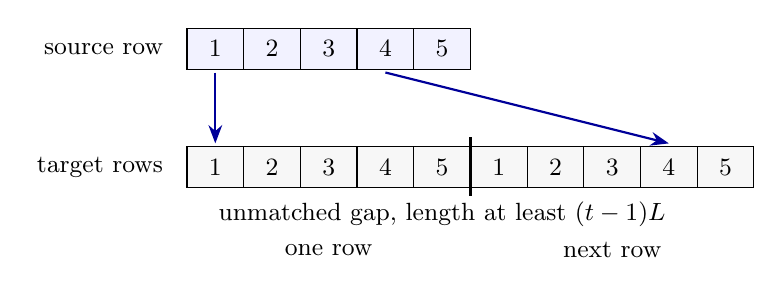
\begin{tikzpicture}[x=.72cm,y=.75cm,>=Stealth,font=\small]
 \node[anchor=east] at (-.25,2) {source row};
 \node[anchor=east] at (-.25,0) {target rows};
 \foreach \i in {0,...,4} {
   \draw[fill=blue!5] (\i,1.65) rectangle ++(1,.7);
   \pgfmathtruncatemacro{\tag}{\i+1}
   \node at (\i+.5,2) {$\tag$};
 }
 \foreach \i in {0,...,9} {
   \draw[fill=black!3] (\i,-.35) rectangle ++(1,.7);
   \pgfmathtruncatemacro{\tag}{mod(\i,5)+1}
   \node at (\i+.5,0) {$\tag$};
 }
 \draw[very thick] (5,-.5)--(5,.5);
 \draw[->,thick,blue!60!black] (.5,1.6)--(.5,.4);
 \draw[->,thick,blue!60!black] (3.5,1.6)--(8.5,.4);
 \draw[<->] (.5,-.8)--(8.5,-.8);
 \node[fill=white,inner sep=2pt] at (4.5,-.8)
   {unmatched gap, length at least $(t-1)L$};
 \node at (2.5,-1.4) {one row};
 \node at (7.5,-1.4) {next row};
\end{tikzpicture}

\caption{Two consecutive matches from one source row enter different target
rows. The labels are child tags. The open target interval between the arrows
is unmatched and contains at least $(t-1)L$ positions. The drawing shows
$t=5$ schematically; only the two relevant matches are shown.}
\label{fig:split-row}
\end{figure}

\section{A circle construction with denominator resets}\label{sec:masks}

We now construct the first family of words. A translation subgroup will
move long lists of rows at low edit cost, while a simultaneous half-turn
will remain separated under every alignment. After proving separation, we derive a common analytic comparison and verify
its arithmetic hypothesis for these translations. The tags will then be
replaced by binary blocks in the next section.

\subsection{Translated rows on a finite circle}
Fix a sufficiently large integer $h$. Choose $h^2$ distinct primes
$p_{\ell k}\in[h^3,2h^3]$, for $1\leq\ell,k\leq h$. Here $\pi(x)$
denotes the number of primes at most $x$. The estimate
$\pi(2x)-\pi(x)>3x/(5\log x)$ for sufficiently large $x$
\cite[Corollary~3]{RosserSchoenfeld1962} supplies this many primes for every
sufficiently large $h$. Put
\begin{equation}\label{mask:parameters}
 P_\ell=\prod_{k=1}^h p_{\ell k},\qquad
 M=2\prod_{\ell=1}^hP_\ell,\qquad R=h^{2h},\qquad
 G=(M^{-1}\mathbb Z)/\mathbb Z.
\end{equation}
The factor two puts the half-turn in the finite grid $G$.

At level $\ell$ the child set is
\[
 J_\ell=\{(k,b):1\leq k\leq h,\ 0\leq b<p_{\ell k}\},
 \qquad t_\ell=\sum_kp_{\ell k},
\]
with a fixed order. For a residue vector
$z\in\prod_k\mathbb Z/p_{\ell k}\mathbb Z$, define the additive maps
\begin{equation}\label{mask:gamma}
 \sigma_\ell(z)=\sum_k\frac{z_k}{p_{\ell k}},\qquad
 \gamma_{\ell,(k,b)}(z)=\sigma_\ell(z)+\frac{bz_k}{p_{\ell k}}
 \quad\text{in }G.
\end{equation}
For an integer $a$, write $z(a)$ for its vector of residues at this level.
By the Chinese remainder theorem, $a\bmod P_\ell$ runs through every $z$.

Set $r_0=1$ and $r_\ell=t_\ell r_{\ell-1}$. A state
$v\in G^{r_\ell}$ is a tuple $(v_j)_{j\in J_\ell}$ with
$v_j\in G^{r_{\ell-1}}$. For $\theta\in G$, write $\theta\mathbf1$ for the
vector whose every coordinate is $\theta$. At level zero, $S_0(v)$ is the length-$M$ binary word with
bit at position $b\in\{0,\ldots,M-1\}$ equal to
\[
 \mathbf1_{[0,1/2)}(b/M-v),
\]
where the interval is read modulo one. Thus $S_0(v)$ records $M/2$
consecutive sites of the circle.

For $\ell\geq1$, define $S_\ell(v)$ by concatenating, for
$a=0,\ldots,RP_\ell-1$, the row
\begin{equation}\label{mask:word}
 \mathop{\Vert}_{j\in J_\ell}
 [j,S_{\ell-1}(v_j+\gamma_{\ell,j}(z(a))\mathbf1)].
\end{equation}
Here $\Vert$ means concatenation in the fixed order, and $[j,U]$ attaches
the tag $j$ to every letter of $U$. The tags are part of the alphabet, so a
match must preserve the child index. All level-$\ell$ words have length
\begin{equation}\label{mask:length}
 L_0=M,\qquad L_\ell=RP_\ell t_\ell L_{\ell-1}.
\end{equation}
At level $h$ the alphabet has size $A=2r_h$. Injectivity of the map from
states to words is not required.

The following subgroup records the translations that move row indices:
\begin{equation}\label{mask:subgroup}
 C_0=\{0\},\qquad
 C_\ell=C_{\ell-1}^{J_\ell}+
 \{(\gamma_{\ell,j}(z)\mathbf1)_{j\in J_\ell}:
        z\in\textstyle\prod_k\mathbb Z/p_{\ell k}\mathbb Z\}.
\end{equation}
For a leaf coordinate $i$, let $e_i(\theta)$ have value $\theta$ there
and zero in the other coordinates.

\begin{lemma}[Cheap translations]\label{mask:cheap}
For every $0\leq\ell\leq h$, every $v\in G^{r_\ell}$, and every
$c\in C_\ell$,
\begin{equation}\label{mask:cheap-subgroup}
 \ED(S_\ell(v),S_\ell(v+c))\leq\frac{2\ell L_\ell}{R}.
\end{equation}
At the top level, for every leaf $i$ and $1\leq a\leq M/2$,
\begin{equation}\label{mask:cheap-leaf}
 \ED(S_h(v),S_h(v+e_i(a/M)))\leq\frac{2aL_h}{Mr_h}.
\end{equation}
Both estimates hold at every base state $v$.
\end{lemma}
\begin{proof}
For a translation from the second summand of~\eqref{mask:subgroup}, choose
its row shift $q\in\{0,\ldots,P_\ell-1\}$ by the Chinese remainder
theorem. Additivity of~\eqref{mask:gamma} identifies the rows after this
shift. Deleting $q$ rows at one end and inserting $q$ at the other costs
at most $2L_\ell/R$. For a translation in the first summand, apply the
previous-level bound inside each child block of each row. Its total cost is
at most $2(\ell-1)L_\ell/R$. These bounds hold at every state, so the
triangle inequality combines them at the intermediate state and proves
\eqref{mask:cheap-subgroup} by induction.

A leaf occupies exactly the fraction $1/r_h$ of the root word, in copies of
$S_0$. Shifting its half-circle by $a/M$, for $a\leq M/2$, changes exactly
$2a$ bits in each copy. Substituting those bits, with every tag unchanged,
proves~\eqref{mask:cheap-leaf}.
\end{proof}

\subsection{A scalar cost and separation under arbitrary alignments}
The subgroup can choose different row translations at successive levels.
To measure how much of a uniform phase survives those choices, define
\begin{equation}\label{mask:phase-cost}
 D_0(\theta)=\|\theta\|_{\mathbb R/\mathbb Z},\qquad
 D_\ell(\theta)=\min_z\frac1{t_\ell}\sum_{j\in J_\ell}
        D_{\ell-1}(\theta+\gamma_{\ell,j}(z)).
\end{equation}
The minimum exists because its set is finite. These functions are symmetric
and subadditive: negate a minimizing residue vector for symmetry, and add
two minimizing vectors before using the preceding subadditivity inequality.
The zero vector also shows $0\leq D_\ell\leq1/2$.

\begin{lemma}[Word separation]\label{mask:separation}
For every $0\leq\ell\leq h$, $v\in G^{r_\ell}$, and $\theta\in G$,
\begin{equation}\label{mask:separation-bound}
 r_{L_\ell}(S_\ell(v),S_\ell(v+\theta\mathbf1))
 \geq\frac{2^{-\ell}}4L_\ell D_\ell(\theta).
\end{equation}
\end{lemma}
\begin{proof}
At level zero let $E$ be the deficit. In a matching of $M-E$ pairs, the
$k$th selected position on either side lies between $k$ and $k+E$, so each
matched pair has displacement at most $E$. The Hamming distance of the two
half-circle words is $2M\|\theta\|_{\mathbb R/\mathbb Z}$. A position where
their bits disagree is either unmatched in the source or matched across a
transition of the target word. The target has at most two transitions in
its linear ordering, and at most $4E$ positions lie within distance $E$ of
them. Thus the Hamming distance is at most $E+4E$. It follows that
$E\geq2MD_0(\theta)/5\geq MD_0(\theta)/4$.

Suppose the assertion holds at level $\ell-1$. Fix a longest common
subsequence matching of the level-$\ell$ words. Let $t=t_\ell$ and
$L=L_{\ell-1}$. If a source row has all its matches in a target row with
indices $a,a'$, respectively, its child $j$ can match only child $j$ in
that target row. Their phase difference is
$(\theta+\gamma_{\ell,j}(z(a'-a)))\mathbf1$. By induction, the number of
source positions lost in this row is at least
\[
 \frac{2^{-(\ell-1)}}4L\sum_j
 D_{\ell-1}(\theta+\gamma_{\ell,j}(z(a'-a)))
 \geq\frac{2^{-(\ell-1)}}4tL D_\ell(\theta).
\]
A row with no matches loses every source position and satisfies the same
bound. Hence Lemma~\ref{pre:tagged-rows} applies with
$A=2^{-(\ell-1)}D_\ell(\theta)/4\leq1/8$. Since $t\geq4$, its denominator
$1+tA/(t-1)$ is less than two. We obtain a deficit at least
$AL_\ell/2$, which is~\eqref{mask:separation-bound}.
\end{proof}

The remaining geometric question is now one-dimensional: how small can
$D_h(1/2)$ be? The next descent gives the quantitative answer. It is here
that the prime groups and their complete residue lists enter the proof.

\subsection{Keeping a nonzero phase through the descent}
\begin{lemma}[Denominator resets]\label{mask:reset}
For all sufficiently large $h$,
\begin{equation}\label{mask:reset-bound}
 D_h(1/2)\geq4^{-h}h^{-h/2-O(\sqrt h)-4h/100},
\end{equation}
with an absolute implicit constant.
\end{lemma}
\begin{proof}
At a level $\ell$, choose a minimizing residue vector $z$ in
\eqref{mask:phase-cost} and let $s=|\{k:z_k\ne0\}|$. If $z_k\ne0$,
multiplication by $z_k$ permutes the $p_{\ell k}$ grid points. For every
translate of that grid, symmetry and subadditivity give
\[
 D_{\ell-1}(1/p_{\ell k})
 \leq D_{\ell-1}(x+b/p_{\ell k})+
       D_{\ell-1}(x+(b+1)/p_{\ell k}).
\]
Averaging over $b$ says that the average cost in this child group is at
least $D_{\ell-1}(1/p_{\ell k})/2$. Its weight in the row is
$p_{\ell k}/t_\ell\geq1/(2h)$. Summing over active groups proves, when
$s>0$, the reset option
\begin{equation}\label{mask:reset-option}
 D_\ell(\theta)\geq\frac{s}{4h}
       \min_{k:z_k\ne0}D_{\ell-1}(1/p_{\ell k}).
\end{equation}
If $s<\sqrt h$, the inactive groups have total weight at least
$(h-s)/(2h)\geq1/4$ for large $h$. They all have phase
$\theta+\sigma_\ell(z)$, so there is also the option
\begin{equation}\label{mask:inactive-option}
 D_\ell(\theta)\geq\tfrac14D_{\ell-1}(\theta+\sigma_\ell(z)).
\end{equation}

Set $K=\lfloor h/100\rfloor$ and start at level $h$ with phase $1/2$.
At entry to level $\ell$, maintain a nonzero phase whose reduced denominator
is a product of at most $K$ distinct primes, all equal to two or belonging
to levels strictly above $\ell$. The initial phase has this property.

Use~\eqref{mask:reset-option} whenever $s\geq\sqrt h$. Use it also when
$s<\sqrt h$ but the current denominator count plus $s$ exceeds $K$.
In the latter case $s>0$, so the option is available. Continue at a prime
reciprocal attaining its minimum. A reset restores the count to one and
leaves a nonzero phase with a prime from the current level.

In every other case use~\eqref{mask:inactive-option}. If the current phase
is $a/Q$ in lowest terms, then $Q>1$. The new summand has denominator
dividing a product $P$ of active current-level primes, with $\gcd(Q,P)=1$.
If $a/Q+b/P$ were an integer, reduction of $aP+bQ$ modulo $Q$ would give
$aP\equiv0\pmod Q$, impossible. The resulting nonzero phase has at most
the old denominator count plus $s$ factors. Thus the invariant is preserved.

Only $O(\sqrt h)$ resets have $s<\sqrt h$. For each such reset, take the
interval of steps since the preceding reset of either kind, or since the
start. Its initial count is one. Overflow implies that the sum of its small
supports, including the last one, exceeds $K-1$. These intervals are
disjoint, and their total support sum is at most $h\sqrt h$. The number $q$
of small resets therefore satisfies
\[
 q\leq\frac{h\sqrt h}{K-1}=O(\sqrt h).
\]
This count remains valid when large resets occur between small ones.

A large reset costs a factor at least $1/(4\sqrt h)$, an inactive step at
least $1/4$, and a small reset at least $1/(4h)$. Their product is at least
$4^{-h}h^{-h/2-q/2}$. At level zero the nonzero phase has at most $K$
denominator primes, each at most $2h^3\leq h^4$. Its distance to zero is
therefore at least $h^{-4K}$. Multiplying the factors and using
$K\leq h/100$ gives~\eqref{mask:reset-bound}.
\end{proof}

Lemmas~\ref{mask:separation} and~\ref{mask:reset} give a pointwise half-turn
deficit at least $L_hh^{-(0.54+o(1))h}$. The exponential factors $8^{-h}$
are absorbed by the $o(1)h$ term on this logarithmic scale. We next check
that the cheap subgroup forces the large frequency size needed to compare
this separation with an $\ell_1$ image.

\subsection{A common analytic comparison for circle shifts}

The word construction has supplied cheap translations and an expensive
half-turn. We now derive the inequality that compares those costs in an
arbitrary $\ell_1$ image. The proof is stated for any finite circle product;
the next subsection will verify its arithmetic hypothesis for the translation
subgroup $C_h$.

For a finite set $X$ and $A\subset X$, write
$\delta_A(x,y)=|\mathbf1_A(x)-\mathbf1_A(y)|$. The finite cut
representation of $\ell_1$ distances is standard
\cite[Section~4]{LinialLondonRabinovich1995}. We include the summability
argument because an $\ell_1$ target may have infinitely many coordinates.

\begin{lemma}[Finite cut representation]\label{pre:cuts}
For $f:X\to\ell_1$ with $X$ finite, there are nonnegative coefficients
$a_A$ on the nonempty proper subsets of $X$ such that
\[
 \|f(x)-f(y)\|_1=\sum_A a_A\delta_A(x,y),\qquad
 \sum_Aa_A\leq\sum_{\{x,y\}\subset X}\|f(x)-f(y)\|_1.
\]
\end{lemma}
\begin{proof}
For real $s,t$,
$|s-t|=\int_{\mathbb R}|\mathbf1_{s>u}-\mathbf1_{t>u}|\,du$.
Apply this to each coordinate of $f$ and group threshold sets that define
the same subset of $X$. Empty and full cuts contribute zero. Every other
cut separates some unordered pair, so its weight is counted at least once
in the displayed pair sum, which is finite. Nonnegative sums and integrals
may be interchanged, giving the representation and the bound.
\end{proof}

For this common lemma, let $M\geq2$ be any even integer,
$G=(M^{-1}\mathbb Z)/\mathbb Z$, and $V=G^r$ for
$r\geq1$. For a map $F:V\to\ell_1$ define its averaged displacement by
\[
 \Delta_F(a)=\E_{v\in V}\|F(v+a)-F(v)\|_1.
\]
All averages on finite groups in this paper are uniform. Represent a
character of $V$ as
$\chi_\alpha(v)=\exp(2\pi\mathrm i\sum_i\alpha_i v_i)$, choosing each
integer $\alpha_i$ with $|\alpha_i|\leq M/2$. Either representative at an
endpoint gives the same absolute value. Put
$T(\alpha)=\sum_i|\alpha_i|$ and
$\mathcal D_M=\{1,2,4,\ldots\}\cap[1,M/2]$.
For $\theta\in G$, write $\theta e_i$ for the vector in $V$ with value
$\theta$ in coordinate $i$ and zero elsewhere.

\begin{lemma}[Weighted finite-circle inequality]\label{pre:weighted-circle}
Let $H\leq V$, let $w=(1/2,\ldots,1/2)\in V$, and suppose $B>0$ satisfies
\begin{equation}\label{pre:branching-premise}
 \chi_\alpha|_H=1,\quad \chi_\alpha(w)\ne1
 \quad\Longrightarrow\quad T(\alpha)\geq B.
\end{equation}
For every $F:V\to\ell_1$ there are nonnegative weights $\omega_\alpha$ with
\begin{equation}\label{pre:fourier}
 \Delta_F(a)=\sum_\alpha\omega_\alpha|1-\chi_\alpha(a)|^2
 \qquad(a\in V).
\end{equation}
Writing $H^\perp=\{\alpha:\chi_\alpha|_H=1\}$, these weights satisfy
\begin{align}
 \sum_{\alpha\notin H^\perp}\omega_\alpha
   &=\tfrac12\E_{u\in H}\Delta_F(u),\label{pre:off-mass}\\
 4\sum_\alpha\omega_\alpha T(\alpha)
   &\leq\sum_{i=1}^r\sum_{a\in\mathcal D_M}
        \frac Ma\Delta_F((a/M)e_i).\label{pre:weighted-mass}
\end{align}
Consequently
\begin{equation}\label{pre:displacement}
 \Delta_F(w)\leq2\E_{u\in H}\Delta_F(u)
 +\frac1B\sum_{i=1}^r\sum_{a\in\mathcal D_M}
        \frac Ma\Delta_F((a/M)e_i).
\end{equation}
\end{lemma}
\begin{proof}
For a scalar function $g$ on $V$, normalized Fourier coefficients and
Parseval give
\[
 \E_v|g(v+a)-g(v)|^2
 =\sum_\alpha|\widehat g(\alpha)|^2|1-\chi_\alpha(a)|^2.
\]
For $g=\mathbf1_A$ its squared difference is the cut distance. Multiply
by the coefficients of Lemma~\ref{pre:cuts} and sum over cuts. This gives
\eqref{pre:fourier} with
$\omega_\alpha=\sum_Aa_A|\widehat{\mathbf1_A}(\alpha)|^2\geq0$.
The sums are finite after grouping cuts. Since a nontrivial character has
mean zero on a finite subgroup, the mean of $|1-\chi_\alpha(u)|^2$ on $H$
is two off $H^\perp$ and zero on it. This proves~\eqref{pre:off-mass}.

For each nonzero coordinate, take the largest power of two
$a\leq M/(2|\alpha_i|)$. It belongs to $\mathcal D_M$ and obeys
\[
 \frac14<\frac{a|\alpha_i|}{M}\leq\frac12,
 \qquad |1-e^{2\pi\mathrm i a\alpha_i/M}|^2\geq2,
 \qquad \frac Ma\geq2|\alpha_i|.
\]
That single scale contributes at least $4|\alpha_i|$. Sum over coordinates
and then against the nonnegative Fourier weights to obtain
\eqref{pre:weighted-mass}.

The half-turn multiplier is zero or four. Its detecting frequencies off
$H^\perp$ contribute at most $4\sum_{\alpha\notin H^\perp}\omega_\alpha$.
By~\eqref{pre:branching-premise}, the remaining ones contribute at most
$(4/B)\sum_\alpha\omega_\alpha T(\alpha)$. The two preceding bounds give
\eqref{pre:displacement}. Equivalently, the same estimates prove that
inequality for each character multiplier separately and then sum it with
nonnegative weights. Thus the lemma supplies both the weighted-mass and
the termwise-displacement forms of the comparison.
\end{proof}

The hypothesis~\eqref{pre:branching-premise} is the only arithmetic input
to this lemma. We shall prove it from the prime translations of each
construction. The inequalities themselves concern averages over all base
states; they impose no pointwise condition on individual Fourier weights.


\subsection{Prime groups force leaf frequency}
Return to the value of $M$ and the grid $G$ in~\eqref{mask:parameters}.
Put $r=r_h$, $V=G^r$, $w=\tfrac12\mathbf1$, and $B=(h/2)^h$. For a character
$\chi_\alpha$ choose the centered integer representatives used in
Lemma~\ref{pre:weighted-circle}.

\begin{lemma}[Frequency branching]\label{mask:branching}
If $\chi_\alpha|_{C_h}=1$ and $\chi_\alpha(w)\ne1$, then
\begin{equation}\label{mask:weight}
 \sum_{i=1}^r|\alpha_i|\geq B.
\end{equation}
\end{lemma}
\begin{proof}
View the state coordinates as the leaves of the tree in~\eqref{mask:word}.
At a node let $\beta$ be the sum of the integer leaf frequencies below it,
and at a level-$\ell$ node let $\beta_{(k,b)}$ be its child sums.
At this node, the translation defined by a residue vector through the maps
$\gamma_{\ell,j}$, and set to zero outside the node, belongs to $C_h$ by the
independent child summands in~\eqref{mask:subgroup}. Choosing $z_k=1$ and
all other coordinates zero gives the congruences
\begin{equation}\label{mask:congruence}
 \beta+\sum_{b=0}^{p_{\ell k}-1}b\beta_{(k,b)}
       \equiv0\pmod{p_{\ell k}}\qquad(1\leq k\leq h).
\end{equation}
They are unchanged if a frequency representative is altered by $M$.

Suppose the sum in~\eqref{mask:weight} were less than $B$. Every nonzero
node sum would have absolute value less than $B$. If $q$ distinct
current-level primes divide such a sum, then
\[
 h^{3q}\leq|\beta|<(h/2)^h<h^h,
\]
so $q<h/3$. For every other prime group,~\eqref{mask:congruence} forces a
nonzero child sum in that group. Each nonzero internal node therefore has
at least $h/2$ nonzero children in distinct groups. At the root, the sum is
odd because $\chi_\alpha(w)\ne1$; parity is well defined since $M$ is even.
Iteration gives at least $(h/2)^h$ nonzero integer leaf frequencies,
contradicting the assumed total absolute sum.
\end{proof}

The lemma verifies~\eqref{pre:branching-premise} with $H=C_h$ and
$B=(h/2)^h$. Thus every $F:V\to\ell_1$ satisfies
\begin{equation}\label{mask:fourier-bound}
 \Delta_F(w)\leq2\E_{c\in C_h}\Delta_F(c)+
 \frac1B\sum_{i=1}^r\sum_{a\in\mathcal D_M}\frac Ma
       \Delta_F(e_i(a/M)).
\end{equation}
We now have all three ingredients: the pointwise half-turn separation,
the pointwise cheap translations, and the averaged $\ell_1$ comparison.
The tags still use $2r_h$ letters. The next section supplies the binary
substitution, after which Section~\ref{sec:mask-binary} completes the
numerical distortion estimate.

\section{Two logarithmic-width binary substitutions}
\label{p2:sec:binary-coding}

The circle words use tags to prevent matches between different children.
We now replace each tagged letter by a binary block. The needed property is
a lower bound for the deficit of every pair of equal-length words, with the
same block-width factor as the elementary upper bound. This makes the loss
in distortion absolute, even as the alphabet grows.

\begin{theorem}[Two binary substitutions]\label{code:two-proofs}
Let $\mathcal A$ be a finite alphabet with $A\geq2$ letters. Each of the two
constructions below gives an integer width $w\geq1$ with $w=O(\log(2A))$, an absolute constant
$a>0$, and a map $c:\mathcal A\to\{0,1\}^w$ such that, simultaneously for
every integer $L\geq0$ and all $x,y\in\mathcal A^L$,
\begin{equation}\label{p2:eq:log-code-deficit}
 a w r_L(x,y)\leq r_{wL}(c(x),c(y))\leq w r_L(x,y).
\end{equation}
Here $c$ extends to words by concatenation. For arbitrary finite words,
\begin{equation}\label{p2:eq:log-code-upper}
 \ED(c(x),c(y))\leq w\ED(x,y).
\end{equation}
The code and its width depend only on $\mathcal A$, not on $L$.
\end{theorem}

The two constructions need not give the same code, width, or constant.
Either substitution may be used in either circle construction.
Their lower bounds imply $(a/2)w\ED(x,y)\leq\ED(c(x),c(y))$ at equal
length, by Lemma~\ref{pre:metric}. The lower assertion is made only at
equal input lengths; the upper assertion holds for arbitrary lengths.
The case $L=0$ is immediate. For the upper deficit bound, concatenate the
code blocks of a common subsequence. For~\eqref{p2:eq:log-code-upper},
simulate each letter insertion, deletion, or substitution by at most $w$
bit edits. It remains to prove the lower deficit bound twice.

\subsection{What an arbitrary bit matching tells us}
Both proofs use the same elementary loss accounting. Fix an increasing
matching between two encoded words of common length $wL$, numbering positions
inside each block from $1$ to $w$, and let $E$ be
its number of unmatched positions on either side. In source block $i$, let
$U_i$ count unmatched positions. If the block has any matches, its target
span is the closed interval from its first partner to its last partner;
let $V_i$ count the globally unmatched target positions in that interval.
For a block without matches put $V_i=0$.

The target spans of different source blocks are disjoint, since their
matches occur in strict order. Also, a matched target position inside one
span has its partner in that source block, by monotonicity. Consequently
\begin{equation}\label{p2:eq:code-loss-sums}
 \sum_iU_i=E,\qquad \sum_iV_i\leq E,
 \qquad |\text{target span of }i|=w-U_i+V_i
\end{equation}
when the span is nonempty. For a threshold $0<\theta<1$, call block $i$
good if $U_i,V_i\leq\theta w$. At most $2E/(\theta w)$ blocks fail this
condition. A good block has a nonempty target span of length at most
$(1+\theta)w<2w$, so its matches meet at most three target blocks.

For the probabilistic choices below, write
$H_2(t)=-t\log_2t-(1-t)\log_2(1-t)$ for binary entropy. We use
\begin{equation}\label{p2:eq:entropy}
 \sum_{j\leq t m}\binom mj\leq2^{H_2(t)m}\qquad(0<t<1/2).
\end{equation}
Indeed, with $z=t/(1-t)<1$,
$(1+z)^m\geq z^{tm}\sum_{j\leq tm}\binom mj$, which rearranges to the
display. The indices in the sum are integers.

\subsection{Different-label intervals and a common offset}
\label{p2:sec:code-offset}
The first code separates sufficiently long intervals of differently
labelled codewords. This kind of interval separation already appears in
the inner code of Schulman and Zuckerman
\cite[Section~II-C, Condition~2 and Lemma~2]{SchulmanZuckerman1999}.
We prove the particular binary property needed here, then use one common
offset in every source block to recover a matching of letters.

Choose an integer $m$ and independent uniform binary words of length $m$, one for each
letter, and put $u=\lfloor m/8\rfloor$. We seek an absolute $\delta>0$
such that every pair of length-$u$ intervals from differently labelled
codewords has longest common subsequence at most $(1-\delta)u$.

Choose an absolute $0<\alpha<1/2$ with
$\gamma=1-\alpha-2H_2(\alpha)>0$. For a fixed pair of intervals with
different labels, the probability of a common subsequence of length
$u-\lfloor\alpha u\rfloor$ is at most
\[
 \binom{u}{\lfloor\alpha u\rfloor}^{\!2}
       2^{-u+\lfloor\alpha u\rfloor}\leq2^{-\gamma u}.
\]
For fixed index lists the involved bits are independent, giving the
probability factor;~\eqref{p2:eq:entropy} bounds their number. There are
at most $A^2m^2$ interval pairs. Taking $m$ to be a sufficiently large
absolute multiple of $\log(2A)$ makes the total failure probability less
than one. For sufficiently large $u$,
$u-\lfloor\alpha u\rfloor\leq(1-\alpha/2)u$; absence of a subsequence of
the former length therefore permits $\delta=\alpha/2$. Fix a code with this property. It makes no assertion
about two intervals of the same codeword.

Choose a positive absolute $\eta<1$ small enough that, for every permitted
width,
\begin{equation}\label{p2:eq:code-offset-parameters}
 2\eta m<\delta\lfloor m/8\rfloor.
\end{equation}
For instance choose $\eta<\delta/100$ first and then increase the minimum
width. Fix $x,y\in\mathcal A^L$, $L\geq1$, and an optimal encoded matching
with deficit $E$. Apply~\eqref{p2:eq:code-loss-sums} with $w=m$ and call a
source block good at threshold $\eta$. At most $2E/(\eta m)$ blocks are
not good.

Let $I=\{\lceil m/3\rceil,\ldots,\lfloor2m/3\rfloor\}$ be the integer
middle-third positions. We claim that a matched position in a good block whose relative index lies in $I$ lands
in a target block with the same letter label. Let $p$ be its relative source
index and $q$ the relative index of its target partner. A length-$u$
interval from $p$ fits in either direction inside the source block. At
least one of those directions fits from $q$ inside its target block. Choose
that direction on both sides. Put $U=U_i$ and $V=V_i$ for this good source
block, and trim the last $V$ source positions from the interval, measured
away from the anchor. For any remaining matched position at source distance
$k\leq u-1-V$ from the anchor, its partner is at target distance at most
$k+V\leq u-1$. The difference of the two distances is the number of
intervening unmatched target positions minus the corresponding source
number, and the former is at most $V$. Monotonicity puts the partner on the
chosen side. At most $U$ retained source positions are unmatched. Hence the
two intervals share a subsequence of length at least
\[
 u-U-V\geq u-2\eta m>(1-\delta)u.
\]
The interval property forces equal labels. This argument also applies when
$q$ is at an endpoint of the target block.

Choose one offset $p$ uniformly from $I$, using this same $p$ in every source
block. The minimum width ensures
$|I|\geq m/4$. Retain each good source block whose position at offset $p$
is matched, and assign it the index of the target block containing that
partner. If $B(p)$ blocks are omitted, then
\begin{equation}\label{p2:eq:code-offset-omissions}
 \E_pB(p)\leq\frac{2E}{\eta m}+\frac E{|I|}
       \leq\left(\frac2\eta+4\right)\frac Em.
\end{equation}
All retained assignments identify equal labels, and their target indices
are nondecreasing. We must count the duplicates before turning them into a
strictly increasing letter matching.

For two consecutive retained blocks that were not originally adjacent,
charge a duplicate target index to an omitted source block strictly between
them. The open source-index gaps of consecutive retained pairs are disjoint,
so these duplicates number at most $B(p)$.

For originally adjacent blocks $i,i+1$, put $d_i=U_i+U_{i+1}$. Their two
positions at a common offset are exactly $m$ apart. If both are matched,
their target partners are at least $m-d_i$ apart. If those partners lie in
one target block, the first is therefore in its first $d_i$ positions.
A good block $i$ meets at most three target blocks, and its distinct source
positions have distinct partners. This duplicate event can thus occur for
at most $3d_i$ offsets; it is impossible when $d_i=0$. Since
$\sum_{i=1}^{L-1}d_i\leq2E$, the number $D_{\rm adj}(p)$ of these adjacent
duplicates satisfies
\begin{equation}\label{p2:eq:code-offset-duplicates}
 \E_pD_{\rm adj}(p)\leq\frac{6E}{|I|}\leq\frac{24E}{m}.
\end{equation}
Only linearity of expectation is used; duplicate events need not be
independent.

In a nondecreasing list, removing one item for each consecutive equality
leaves one item for every distinct index. The retained assignments therefore
give an increasing equal-letter subsequence after at most
$B(p)+D_{\rm adj}(p)$ further deletions. Thus
$r_L(x,y)\leq2B(p)+D_{\rm adj}(p)$. Taking expectations gives
\[
 r_L(x,y)\leq\left(\frac4\eta+32\right)\frac Em.
\]
This proves the first construction in Theorem~\ref{code:two-proofs} with
$w=m$ and $a=(4/\eta+32)^{-1}$. All constants were chosen before $L$,
and the estimate has no additive error depending on $L$.

\subsection{Self-overlaps and an anchor at equal relative indices}
\label{p2:sec:code-anchor}
The second code controls a different local event. It rules out a long,
nearly complete matching between two codeword intervals unless their labels
agree and one matched pair has the same index relative to its two block
starts. That anchor will put a strict majority of one source block into a
single target block, making the recovered letter assignments distinct.

Choose an absolute $\epsilon>0$ with
\begin{equation}\label{p2:eq:code-anchor-parameters}
 2H_2(\epsilon)<\tfrac18,\qquad \epsilon<\tfrac1{10}.
\end{equation}
We seek binary codewords of width $M$ with this precise property: every
increasing matching of at least $M/4$ pairs between two codewords, omitting
at most $\epsilon M$ positions in each of its two spanned intervals, has
equal labels and contains a pair at equal relative indices. The two
codewords may have the same label, so this condition controls shifted
self-overlaps as well.

Self-matching is central to synchronization strings
\cite[Sections~6.1--6.2 of the full version]{HaeuplerShahrasbi2017};
related local conditions occur in the Hamming-to-edit construction of
Bhattacharya et al.\ \cite[Section~2.2]{BhattacharyaEtAl2026}. The property
just stated is the particular one we need, and the following argument
proves it directly.

Choose all code bits independently and uniformly. For a fixed pair of
labels, there are at most
\[
 M^4\left(\sum_{j\leq\epsilon M}\binom Mj\right)^2
 \leq M^4 2^{2H_2(\epsilon)M}
\]
candidate index-list pairs: choose four span endpoints and the omitted
positions; the remaining increasing lists determine the matching. Counting
choices of different list lengths only enlarges the bound.

For different labels, a fixed matching of $q\geq M/4$ pairs has equality
probability $2^{-q}$. For the same label and no equal-index pair, form a
graph on the $M$ independent code bits with one edge for each required
equality. It has no loops. Every index occurs at most once in either list,
so the degree, counting incidences, is at most two. A repeated unordered
edge would require reversed index pairs and violate strict increase; even
if double edges were allowed, a nontrivial connected component with $v$
vertices and $e$ edges has $v\geq2$, $e\leq v$, and $v-1\geq e/2$.
Equality of all bits in that component imposes $v-1$ independent binary
constraints. The full equality system therefore has rank at least $q/2$,
so its probability is at most $2^{-q/2}\leq2^{-M/8}$.

The probability of any violation of the local property is at most
\[
 A^2M^4 2^{(2H_2(\epsilon)-1/8)M}.
\]
By~\eqref{p2:eq:code-anchor-parameters}, this is less than one for $M$ a
sufficiently large absolute multiple of $\log(A+1)$. Fix such codewords.

Now take an optimal matching of $c(x),c(y)$ with deficit $E$, and use
\eqref{p2:eq:code-loss-sums} with $w=M$ and threshold $\epsilon$. At most
$2E/(\epsilon M)$ source blocks are not good. A good block has at least
$(1-\epsilon)M$ matches in a span meeting at most three target blocks.
One target block receives at least $(1-\epsilon)M/3\geq M/4$ of them.
Restrict to matches between this source and target block. A position
between the first and last restricted matches on either side, if globally
matched, is still in the restricted matching: monotonicity places its
partner between the opposite endpoints. Hence the omissions in the two
restricted spans are bounded by $U_i,V_i$. The local property gives equal
labels and an anchor at equal relative indices.

Put $b=\lfloor\epsilon M\rfloor$. Both losses of the good block are at
most $b$. Measure target indices relative to the fixed start of the chosen
target block, even for matches outside it. Relative to the anchor, the
displacement of any match from equal relative indices is the difference
between the intervening unmatched counts. Its absolute value is at most
$2b$. Every matched source index in
$\{2b+1,\ldots,M-2b\}$ therefore still lands in the chosen target block.
At most $b$ of these $M-4b$ positions are unmatched. The chosen block
receives at least
\[
 M-5b\geq(1-5\epsilon)M>M/2
\]
matches. Two good source blocks cannot choose the same target block, since
their matched target positions are disjoint. Their chosen target indices
are increasing by monotonicity. The good blocks thus give an equal-letter
subsequence, proving
\[
 r_L(x,y)\leq\frac{2E}{\epsilon M}.
\]
This is the second construction with $w=M$ and $a=\epsilon/2$, completing
Theorem~\ref{code:two-proofs}.

\subsection{Relation to the earlier alphabet reduction}
The existence order in Theorem~\ref{code:two-proofs} has a close predecessor.
Theorem~1.1 of the full version of Bhattacharya, Dey, Goldenberg, and Kouck\'y
\cite{BhattacharyaDeyGoldenbergKoucky2024} states an alphabet reduction for
normalized insertion--deletion distance, with each distance divided by the
sum of the lengths of its two arguments.
The construction used to prove that theorem is a fixed block substitution
$C:\mathcal A\to Q^k$ in Section~3.2.1 and Lemma~3.3. With approximation
parameter $1/8$, the target alphabet $Q$ has absolute size $q\geq2$, and
$k=O(\log(2A))$. Their stated normalized bounds, applied to that
construction, give
\begin{equation}\label{code:prior-indel}
 \tfrac78 k\Delta(x,y)\leq\Delta(C(x),C(y))\leq k\Delta(x,y).
\end{equation}
Indeed, the total encoded length is $k(|x|+|y|)$, so the normalizing factor
cancels. When both words are empty, the unnormalized inequalities are
immediate.

For clarity, here is the elementary binary step in this comparison.
Give the $q$ target letters distinct $t=\lceil\log_2q\rceil$ bit labels and
encode a letter $a$ by
$j(a)=11\,0\,a_1\,0\cdots a_t\,0$, of fixed width $v=2t+3$.
The string $11$ occurs exactly at a block start. In any increasing bit
matching, let $e$ count unmatched positions in the two words together.
Then at most $e$ source blocks fail to
be fully matched to consecutive target positions: charge a block either
to one of its unmatched source bits or, if all its bits are matched, to
an unmatched target position skipped between consecutive partners. The
charged gaps of different source blocks are disjoint. The same bound holds
on the target side. A fully and consecutively matched block begins at a
genuine target block start, by the unique $11$, so it matches an entire
equal block that is itself good on the target side. Conversely, every good
target block is paired this way. The good blocks therefore give a letter matching with total loss at most
$2e$. Minimizing over bit matchings proves
\[
 \tfrac12\Delta(u,z)\leq\Delta(j(u),j(z))\leq v\Delta(u,z)
\]
for arbitrary finite words; the upper bound simulates letter edits.

The composite $j\circ C$ is a single binary substitution of width $w=vk$.
Combining this inequality with~\eqref{code:prior-indel} gives
$\Delta(jC(x),jC(y))\geq(7/(16v))w\Delta(x,y)$. At equal lengths this is
the deficit lower factor $7/(16v)$, and for ordinary edit distance it gives
the lower factor $7/(32v)$; bitwise simulation gives the upper factor one.
This deduction uses the earlier stated theorem and its block construction.
The two proofs above establish the stated binary bounds directly and exhibit
distinct ways to recover a letter matching.

\section{The first binary obstruction}\label{sec:mask-binary}

We return to the words $S_h$ and parameters $M,R,C_h$ from
Section~\ref{sec:masks}; here $w=\tfrac12\mathbf1$ again denotes the
half-turn in $G^{r_h}$. The words use an alphabet of size $A=2r_h$.
Apply the first construction of
Theorem~\ref{code:two-proofs}, with width $b_h\leq C\log(2A)$ and lower
deficit factor $a_{\rm off}b_h$, where $a_{\rm off}>0$ is absolute.
Let $X_h(v)=c(S_h(v))$ and $n_h=b_hL_h$. The code is fixed for this
alphabet and applies at the common length $L_h$.

The code lower bound, word separation, and denominator reset estimate give,
for all sufficiently large $h$ and every state $v$,
\begin{equation}\label{mask:binary-far}
 \ED(X_h(v),X_h(v+w))\geq n_h h^{-0.75h}.
\end{equation}
Indeed, the normalized deficit before coding is at least
$h^{-(0.54+o(1))h}$, and the fixed factor $a_{\rm off}$ is absorbed by the
slack to $0.75$. Simulating each letter edit with at most $b_h$ bit edits
in Lemma~\ref{mask:cheap} also gives
\begin{align}
 \ED(X_h(v),X_h(v+c))&\leq n_h\frac{2h}{R}
        &&(c\in C_h),\label{mask:binary-subgroup}\\
 \ED(X_h(v),X_h(v+e_i(a/M)))&\leq n_h\frac{2a}{Mr_h}
        &&(1\leq a\leq M/2).\label{mask:binary-leaf}
\end{align}
These bounds hold at every base state. The state map need not be injective;
\eqref{mask:binary-far} guarantees precisely the distinct pairs needed.

Let $f$ be any embedding of the finite image of $X_h$ into $\ell_1$, with
distortion $D$. Scale it so that
\[
 \ED(x,y)/D\leq\|f(x)-f(y)\|_1\leq\ED(x,y).
\]
This uses the maximum expansion on the finite image and does not assume
that the infimum of distortions is attained. Apply~\eqref{mask:fourier-bound}
to $F=f\circ X_h$. Each coordinate-scale term, after multiplication by
$M/a$, is at most $2n_h/r_h$. The pointwise edit bounds therefore imply
\begin{equation}\label{mask:distortion-estimate}
 \frac{h^{-0.75h}}D\leq\frac{4h}{R}
              +\frac{2|\mathcal D_M|}{B}.
\end{equation}
Here $|\mathcal D_M|=O(\log M)$ and $\log M=O(h^2\log h)$.
Since $R=h^{2h}$ and $B=(h/2)^h$, the right side is at most
$C2^h h^{-h}h^2\log h$ for large $h$. Hence
\begin{equation}\label{mask:distortion}
 D\geq c\,2^{-h}\frac{h^{h/4}}{h^2\log h}\geq h^{0.1h}.
\end{equation}

Finally $t_\ell\leq2h^4$ gives $\log r_h=O(h\log h)$ and
$b_h=O(h\log h)$. The exact recurrence~\eqref{mask:length} yields
\begin{equation}\label{mask:length-bound}
 \log n_h=\log b_h+\log M+
 \sum_{\ell=1}^h(\log R+\log P_\ell+\log t_\ell)
 \leq C_{\rm len}h^2\log h
\end{equation}
with an absolute constant $C_{\rm len}$. Thus every sufficiently large
integer $h$ supplies a binary same-length obstruction with distortion at
least $h^{0.1h}$ and logarithmic length at most $C_{\rm len}h^2\log h$.
After the second construction, Section~\ref{sec:assembly} will convert each
such family into witnesses for every sufficiently large cap.

\section{Excluded-coordinate translations on a finite circle}
\label{sec:excluded-coordinate}\label{sec:excluded}

We now construct a second family of hard binary words.  The parameter is a
sufficiently large integer $m$; the eventual distortion is at least
$m^{m/4}$, while the logarithm of the word length is $O(m^2\log m)$.
At each level there is one prime for each of the $m$ child indices.  The
translation associated with that prime acts on every child except its own.
This omission has two
uses.  A small phase cost will force most translation coordinates to vanish,
whereas a frequency annihilating all the translations and detecting the
half-turn must have large total absolute leaf frequency. The proof of this
frequency bound assumes the total is small and forces branching through
too many children.  We first prove the phase assertion, then realize it
by words and compare it with the frequency assertion.

\subsection{The translation pattern and its phase cost}

Write $\mathbb T=\mathbb R/\mathbb Z$ for the circle of circumference one,
and let $\|z\|_{\mathbb T}$ denote the distance of $z$ from zero.  Set $h=m$.
We need $hm=m^2$ primes, all distinct across all levels, satisfying
\begin{equation}\label{eq:exc-primes}
 m^3<p_{\ell,i}\le m^5,
 \qquad 1\le\ell\le h,\quad 1\le i\le m.
\end{equation}
The following count uses the central binomial coefficient and Legendre's
factorial valuation formula in the manner of Erd\H{o}s \cite{Erdos1932},
who attributes the underlying ideas to Landau.  The central term is the
largest of the $2n+1$ binomial coefficients summing to $4^n$, so
\[
 \binom{2n}{n}\ge\frac{4^n}{2n+1}.
\]
In the valuation formula for $\binom{2n}{n}$, each term
$\lfloor2n/p^j\rfloor-2\lfloor n/p^j\rfloor$ is zero or one.  Thus the
exponent of $p$ is at most $\lfloor\log_p(2n)\rfloor$, and each prime
contributes a factor at most $2n$.  Writing $\pi(x)$ for the number of
primes at most $x$, we obtain
\[
 \binom{2n}{n}\le (2n)^{\pi(2n)}.
\]
Taking logarithms and then $n=\lfloor m^5/2\rfloor$ gives
$\pi(m^5)\ge c m^5/\log m$ for an absolute $c>0$ and all sufficiently
large $m$.  Since $\pi(m^3)\le m^3$, the interval $(m^3,m^5]$ contains
at least $m^2$ primes once $m$ is large enough.  Fix such a choice.

For each level put
\begin{equation}\label{eq:exc-translations}
 P_\ell=\prod_{i=1}^m p_{\ell,i},\qquad
 u_{\ell,i}(s)=\frac{s}{p_{\ell,i}}\pmod1,\qquad
 c_{\ell,i}(s)=\sum_{j\ne i}u_{\ell,j}(s).
\end{equation}
The parameter $s$ is taken modulo $P_\ell$.  By the Chinese remainder
theorem, $(u_{\ell,i}(s))_{i=1}^m$ runs through the full product of the
prime-order subgroups.  In particular, one coordinate can be prescribed
while all the others are set to zero.  Each $c_{\ell,i}$ is a homomorphism.
If only $u_{\ell,i}$ is nonzero, its value is added to all children except
child $i$.

The scalar cost of a phase after $\ell$ levels is
\begin{equation}\label{eq:exc-rho}
 \rho_0(z)=\|z\|_{\mathbb T},\qquad
 \rho_\ell(z)=\min_{s\bmod P_\ell}
       \frac1m\sum_{i=1}^m
          \rho_{\ell-1}\bigl(z+c_{\ell,i}(s)\bigr)
       \quad(1\le\ell\le h).
\end{equation}
These functions are defined on all of $\mathbb T$.  Each minimum is over a
finite set.
They are symmetric and subadditive: negate a minimizing parameter for
symmetry, and add minimizing parameters for two inputs and use the preceding
subadditivity term by term.  The zero parameter shows inductively that, for
$1\le\ell\le h$,
\[
 \rho_\ell(0)=0,\qquad
 0\le \rho_\ell(z)\le \rho_{\ell-1}(z)
       \le\|z\|_{\mathbb T}\le\frac12.
\]

The next lemma quantifies what the omitted coordinate prevents.  Its input
phase has a small order relatively prime to the primes still available in
the recurrence.  The phases followed during the proof can have much larger
orders.

\begin{lemma}[Small-order phases remain costly]\label{lem:exc-small-cost}
For $0\le\ell\le h$, put
\[
 F_\ell=m^{-\ell/4-100m^{3/4}}.
\]
For all sufficiently large $m$, the following holds for every
$0\le\ell\le h$.  If $z\in\mathbb T$ is nonzero, has finite order
$q\le m^{10}$, and satisfies
$\gcd(q,\prod_{a=1}^{\ell}P_a)=1$, then
\begin{equation}\label{eq:exc-phase-lower}
 \rho_\ell(z)\ge F_\ell.
\end{equation}
The empty product in the case $\ell=0$ is one.
\end{lemma}

\begin{proof}
At height zero a nonzero point of order $q$ has distance at least
$1/q\ge m^{-10}\ge F_0$ for large $m$.  Suppose the lemma is known at all
heights below $\ell\ge1$, and suppose, for a contradiction, that an input
as in the statement satisfies $\rho_\ell(z)<F_\ell$.

We record the bounds that will keep a descent through the recurrence under
control.  Let $a=m^{-1/4}$ and $b_t=4a^{t+1}$ for $t\ge0$.  For
$m\ge32^4$, all $b_t<1$ and
\begin{align}
 \log\prod_{t\ge0}(1-b_t)^{-1}
 &\le \sum_{t\ge0}\frac{b_t}{1-b_t}
 \le \frac{4a}{(1-a)(1-4a)}<\log2,
 \label{eq:exc-product-cost}\\
 m\sum_{t\ge0}b_t
 &=\frac{4m^{3/4}}{1-m^{-1/4}}\le5m^{3/4}.
 \label{eq:exc-support-budget}
\end{align}
We will choose phases $z_0=z,z_1,\ldots,z_\ell$ so that, at time $t$,
\begin{equation}\label{eq:exc-path-invariant}
 \rho_{\ell-t}(z_t)
 <F_\ell\prod_{j<t}(1-b_j)^{-1}<2F_\ell .
\end{equation}
The first inequality holds at $t=0$ by assumption.

Suppose $t<\ell$ and write $r=\ell-t$ for the remaining height.  Choose a
parameter attaining the minimum in $\rho_r(z_t)$, abbreviate
$u_i=u_{r,i}(s)$, and put $U=\sum_i u_i$.  Call an index $i$ small when
\[
 \rho_{r-1}(z_t+U-u_i)<F_{r-1}/2.
\]
The average of these $m$ costs is less than $2F_\ell$ by
\eqref{eq:exc-path-invariant}.  Hence the number of indices that are not
small is at most
\begin{equation}\label{eq:exc-exception-count}
 \frac{4mF_\ell}{F_{r-1}}
   =4m^{1-(t+1)/4}=mb_t.
\end{equation}
This is at most $4m^{3/4}$, so there are at least two small indices for all
large $m$.

If two small indices $i,j$ had $u_i\ne u_j$, symmetry and subadditivity
would give
\[
 \rho_{r-1}(u_i-u_j)
 \le \rho_{r-1}(z_t+U-u_i)+\rho_{r-1}(z_t+U-u_j)
 <F_{r-1}.
\]
The difference is nonzero and its order divides
$p_{r,i}p_{r,j}\le m^{10}$.  That order is relatively prime to
$\prod_{a<r}P_a$, since all level primes are distinct.  The induction
hypothesis at height $r-1$ rules out the displayed inequality.  Therefore
all small indices have the same $u_i$.  Two distinct prime-order subgroups
of $\mathbb T$ intersect only at zero; the presence of two small indices
then implies that every small index has $u_i=0$.

Let $k_t=\#\{i:u_i\ne0\}$.  We have $k_t\le mb_t<m$.  Every zero coordinate
gives the same child phase $z_t+U$; choose
$z_{t+1}=z_t+U$.  The other costs are nonnegative, so
\begin{equation}\label{eq:exc-path-cost}
 \rho_{r-1}(z_{t+1})
 \le\frac{\rho_r(z_t)}{1-k_t/m}
 \le\frac{\rho_r(z_t)}{1-b_t}.
\end{equation}
This proves the first inequality of \eqref{eq:exc-path-invariant} at
$t+1$; its second inequality follows from \eqref{eq:exc-product-cost}.
Thus the descent is justified at every step.  It uses fractions from at
most
\begin{equation}\label{eq:exc-denominator-count}
 \sum_{t=0}^{\ell-1}k_t
 \le m\sum_{t\ge0}b_t\le5m^{3/4}
\end{equation}
distinct level primes, by \eqref{eq:exc-support-budget}.

It remains to compare the terminal phase with its cost.  Let $Q$ be the
product of the primes actually used in the descent.  Then $z_\ell-z$ has
order dividing $Q$, and
\[
 qQ\le m^{10+25m^{3/4}}.
\]
The phase $z_\ell$ is nonzero.  Otherwise the order $q>1$ of $z$ would
divide $Q$, contradicting $\gcd(q,Q)=1$.  Since the order of $z_\ell$
divides $qQ$, we conclude that
\[
 \rho_0(z_\ell)=\|z_\ell\|_{\mathbb T}
 \ge m^{-10-25m^{3/4}}.
\]
But \eqref{eq:exc-path-invariant} gives
\[
 \rho_0(z_\ell)<2F_\ell
   =2m^{-\ell/4-100m^{3/4}}
   <m^{-10-25m^{3/4}}
\]
for sufficiently large $m$, a contradiction.  The induction hypothesis
was used only for the differences $u_i-u_j$.  The selected phases $z_t$
were controlled by their accumulated denominators, without a small-order
assumption on them.
\end{proof}

\subsection{Words whose tags preserve the child index}

We now turn the scalar cost into edit separation.  Put
\begin{equation}\label{eq:exc-size-parameters}
 L=2\prod_{\ell=1}^hP_\ell,\qquad R=m^{2h},\qquad
 \Lambda=[m]^h,\qquad
 G=(L^{-1}\mathbb Z/\mathbb Z)^\Lambda .
\end{equation}
The set $\Lambda$ indexes the leaves of an $m$-ary tree of height $h$:
a node at height $\ell$ is a prefix $a\in[m]^{h-\ell}$, and $ai$ denotes
its child obtained by appending $i$.  The alphabet is
\[
 \mathcal A=\Lambda\times\{0,\ldots,L-1\}\times\{0,1\},
 \qquad J=|\mathcal A|=2Lm^h.
\]
The first two coordinates are symbol tags.  The factor two in $L$ places
the half-turn in the phase group, and every translation
$c_{\ell,i}(s)$ also belongs to this group.

For a state $v\in G$ and an auxiliary phase
$\theta\in L^{-1}\mathbb Z/\mathbb Z$, define $W_a(v,\theta)$ recursively.
At a leaf $a$, it is the length-$L$ word
\begin{equation}\label{eq:exc-leaf-word}
 W_a(v,\theta)=
 \bigl(a,b,\mathbf1_{[0,1/2)}(b/L-v_a-\theta)\bigr)_{b=0}^{L-1},
\end{equation}
where the half-open interval is interpreted on $\mathbb T$.  At height
$\ell\ge1$, concatenate the following rows, each consisting of $m$ child
words:
\begin{equation}\label{eq:exc-internal-word}
 W_a(v,\theta)=
 \mathop{\Vert}_{s=0}^{RP_\ell-1}
 \mathop{\Vert}_{i=1}^{m}
 W_{ai}\bigl(v,\theta+c_{\ell,i}(s)\bigr).
\end{equation}
The symbol $\Vert$ denotes concatenation in the displayed order.  All
height-$\ell$ words have the same length
\begin{equation}\label{eq:exc-length-recurrence}
 N_0=L,\qquad N_\ell=mRP_\ell N_{\ell-1}.
\end{equation}
Write $N=N_h$ and $W(v)=W_{\varnothing}(v,0)$.  Adding a phase $z$ to
every state coordinate below a node has the same effect on its word as
replacing $\theta$ by $\theta+z$: this follows at a leaf from
\eqref{eq:exc-leaf-word}, and then at every height from the concatenation.

\begin{lemma}[Separation under arbitrary alignments]\label{lem:exc-alignment}
For every node $a$ at height $0\le\ell\le h$, every $v\in G$, and every
$\theta,z\in L^{-1}\mathbb Z/\mathbb Z$,
\begin{equation}\label{eq:exc-word-separation}
 r_{N_\ell}\bigl(W_a(v,\theta),W_a(v,\theta+z)\bigr)
 \ge N_\ell 3^{-\ell}\rho_\ell(z).
\end{equation}
\end{lemma}

\begin{proof}
At a leaf, the position tag $b$ forces a matched symbol to use the same
position on both sides.  The two half-circle indicators disagree at
exactly $2L\|z\|_{\mathbb T}$ positions.  Their deficit is therefore
exactly that number, which is at least $L\rho_0(z)$.

Suppose the lemma holds at height $\ell-1$ and fix a longest common
subsequence at height $\ell$, with deficit $E$.  A row in
\eqref{eq:exc-internal-word} has $m$ children of length $N_{\ell-1}$.
Because every symbol carries its leaf tag, a match between these two node
words preserves the child index $i$.  We verify the nonsplit-row hypothesis
of Lemma~\ref{pre:tagged-rows}.

Suppose all matches from a source row with parameter $s$ lie in a target
row with parameter $s'$.  Within child $i$ they form a matching of two full
child words whose phase difference is
$z+c_{\ell,i}(s'-s)$.  By induction, the number of unmatched source
positions in that child is at least
\[
 N_{\ell-1}3^{-(\ell-1)}
       \rho_{\ell-1}\bigl(z+c_{\ell,i}(s'-s)\bigr).
\]
Summing over $i$ and using \eqref{eq:exc-rho}, the source row loses at least
the fraction
\[
 A=3^{-(\ell-1)}\rho_\ell(z)
\]
of its positions.  A row with no matches loses every position and satisfies
the same estimate.  Here $0\le A\le1/2$.  Lemma~\ref{pre:tagged-rows},
with $t=m$ and child length $N_{\ell-1}$, now gives
\[
 E\ge\frac{A N_\ell}{1+mA/(m-1)}
   \ge \frac{A N_\ell}{3}.
\]
For the last inequality we used $m/(m-1)\le2$ and $A\le1$.  This is
\eqref{eq:exc-word-separation}.  Lemma~\ref{pre:tagged-rows} applies to the
chosen arbitrary matching; in particular it permits different nonsplit
source rows to use the same target row.
\end{proof}

Let $w_*\in G$ have every coordinate equal to $1/2$.  All primes in
\eqref{eq:exc-primes} are odd.  The phase $1/2$ has order two, so
Lemmas~\ref{lem:exc-small-cost} and~\ref{lem:exc-alignment}, together with
the phase identity for node words, give the pointwise bound
\begin{equation}\label{eq:exc-halfturn}
 r_N\bigl(W(v),W(v+w_*)\bigr)\ge N3^{-h}F_h
 \qquad(v\in G).
\end{equation}

\subsection{Cheap translations and the binary transfer}

For a node $a$ at height $\ell\ge1$ and $s\bmod P_\ell$, define
$\tau_{a,s}\in G$ by
\[
 (\tau_{a,s})_b=
 \begin{cases}
 c_{\ell,i}(s),&\text{if the leaf $b$ has prefix $ai$},\\
 0,&\text{if $b$ is outside the subtree below $a$}.
 \end{cases}
\]
Let $H\le G$ be the subgroup generated by these vectors over all internal
nodes.  At each fixed node, $s\mapsto\tau_{a,s}$ is a homomorphism.

Fix one height $\ell$ and choose one translation at each node of that
height.  In an occurrence of $W_a(v,\theta)$, adding $\tau_{a,s}$ replaces
row parameter $t$ by $t+s$ in \eqref{eq:exc-internal-word}.  The row list
has period $P_\ell$ and repeats it $R$ times.  Choose $0\le s<P_\ell$.
Deleting the first $s$ rows from the unshifted list and the last $s$ rows
from the shifted list leaves identical words.  The edit cost in this
occurrence is at most
\[
 2s\,mN_{\ell-1}\le \frac{2N_\ell}{R}.
\]
At a fixed height the node occurrences partition the root word.  The
combined cost for all nodes at that height is therefore at most $2N/R$.
Every element of $H$ is a sum of at most $h$ such single-height
translations: $G$ is abelian, sums at one node combine to one parameter,
and the nodes can then be grouped by height.  The edit estimate holds for
every state and every ancestor phase.  Applying it at each intermediate
state and using the triangle inequality gives
\begin{equation}\label{eq:exc-cheap-subgroup}
 \operatorname{ED}\bigl(W(v),W(v+u)\bigr)
 \le\frac{2hN}{R}
 \qquad(v\in G,\ u\in H).
\end{equation}

For a leaf $a\in\Lambda$, write $ze_a$ for the state vector with value $z$
at $a$ and zero elsewhere. This shift changes exactly $2L\|z\|_{\mathbb T}$ symbols in every occurrence
of that leaf word.  Each branching has $m$ equally long children, so the
occurrences of a fixed leaf occupy the fraction $m^{-h}$ of the root word.
Substituting only the changed symbols yields
\begin{equation}\label{eq:exc-cheap-coordinate}
 \operatorname{ED}\bigl(W(v),W(v+ze_a)\bigr)
 \le\frac{2N}{m^h}\|z\|_{\mathbb T}.
\end{equation}
This holds for every $v\in G$, $z\in L^{-1}\mathbb Z/\mathbb Z$, and
$a\in\Lambda$.

Apply the second construction of Theorem~\ref{code:two-proofs}, proved
using anchors at equal relative indices in Section~\ref{p2:sec:code-anchor}, to
$\mathcal A$.  It gives one code
$\mathcal C:\mathcal A\to\{0,1\}^{w}$ with
$w\le C_{\rm code}\log(2J)$ and an absolute $\eta>0$.  Its exact estimates
are
\begin{equation}\label{eq:exc-code-interface}
 \begin{aligned}
 r_{wq}(\mathcal Cx,\mathcal Cy)&\ge\eta w r_q(x,y)
       &&(x,y\in\mathcal A^q),\\
 \operatorname{ED}(\mathcal Cx,\mathcal Cy)
       &\le w\operatorname{ED}(x,y).
 \end{aligned}
\end{equation}
The lower estimate holds simultaneously at every common length $q\ge0$,
with the code fixed before $q$ is chosen; the upper estimate holds for
arbitrary finite words.  Here we use the lower estimate at the common
length $N$.

Set $X(v)=\mathcal C W(v)$ and $n_*=wN$.  The metric comparison
$r_{n_*}\le\operatorname{ED}$ from Lemma~\ref{pre:metric}, the code
estimates, and \eqref{eq:exc-halfturn}--\eqref{eq:exc-cheap-coordinate}
give
\begin{align}
 \frac{\operatorname{ED}(X(v),X(v+w_*))}{n_*}
 &\ge\eta3^{-h}F_h,
 \label{eq:exc-binary-far}\\
 \frac{\operatorname{ED}(X(v),X(v+u))}{n_*}
 &\le\frac{2h}{R},
 \label{eq:exc-binary-subgroup}\\
 \frac{\operatorname{ED}(X(v),X(v+ze_a))}{n_*}
 &\le\frac{2}{m^h}\|z\|_{\mathbb T}.
 \label{eq:exc-binary-coordinate}
\end{align}
All three inequalities hold for every $v\in G$.  The second holds for every
$u\in H$, and the third for every $z\in L^{-1}\mathbb Z/\mathbb Z$ and
$a\in\Lambda$.  In particular, each half-turn pair consists of distinct
words; other repetitions among the state images are allowed.

\subsection{Large total leaf frequency}

It remains to show that the cheap translations prevent an $\ell_1$ map
from preserving the half-turn distance.  Write characters of $G$ as
\[
 \chi_\xi(v)=\exp\!\left(2\pi\mathrm i\sum_{a\in\Lambda}\xi_a v_a\right),
 \qquad
 \xi\in(\mathbb Z/L\mathbb Z)^\Lambda .
\]
For each coordinate choose an integer representative of minimum absolute
value, with either sign allowed in a tie, and put
\begin{equation}\label{eq:exc-frequency-size}
 T(\xi)=\sum_{a\in\Lambda}|\xi_a|.
\end{equation}
Thus $T$ records the total magnitude of the leaf frequencies.  Let
$H^\perp=\{\xi:\chi_\xi(u)=1\text{ for every }u\in H\}$.

\begin{lemma}[Annihilating frequencies that detect the half-turn]
\label{lem:exc-annihilator}
If $\xi\in H^\perp$ and $\chi_\xi(w_*)\ne1$, then
\begin{equation}\label{eq:exc-annihilator-threshold}
 T(\xi)\ge K,\qquad K=m^{3h/4}.
\end{equation}
\end{lemma}

\begin{proof}
For each node $a$, let $t_a$ be the sum of the chosen integer
representatives over all leaves below $a$.  Thus $t_a=\xi_a$ at a leaf,
and $t_a=\sum_i t_{ai}$ at an internal node.  At height $\ell$, the Chinese
remainder theorem permits a parameter with
$u_{\ell,i}=1/p_{\ell,i}$ and all other $u_{\ell,j}=0$.  Its node
translation adds $1/p_{\ell,i}$ to every child other than $i$.  Since
$\xi$ annihilates this translation,
\begin{equation}\label{eq:exc-annihilator-congruence}
 t_a-t_{ai}\equiv0\pmod{p_{\ell,i}}
 \qquad(1\le i\le m).
\end{equation}
This congruence is independent of the integer lifts because every
$p_{\ell,i}$ divides $L$.

The half-turn satisfies $\chi_\xi(w_*)=(-1)^{t_{\varnothing}}$.
Consequently the root sum is odd and is nonzero.  Suppose that $T(\xi)<K$.
Every node sum has absolute value at most $T(\xi)$, hence less than $K$.
At a node with $t_a\ne0$, let $q$ be the number of its level primes
dividing $t_a$.  If $q>0$, distinctness and \eqref{eq:exc-primes} give
\[
 m^{3q}
 <\prod_{p_{\ell,i}\mid t_a}p_{\ell,i}
 \le |t_a|<m^{3h/4}.
\]
Thus $q<h/4$; the same inequality is immediate when $q=0$.
For every other child, \eqref{eq:exc-annihilator-congruence} forces
$t_{ai}\ne0$.  Since $h=m$, each nonzero internal node has at least
$3m/4$ nonzero children.  Starting with the root, this gives at least
$(3m/4)^h$ nonzero leaf coefficients.  These are nonzero integers, so
\[
 T(\xi)\ge(3m/4)^h\ge m^{3h/4}=K
\]
for all sufficiently large $m$, a contradiction.
\end{proof}

\subsection{The distortion and length estimates}

Let $f$ be any injection of the finite set $X(G)$ into $\ell_1$, with
distortion $D$.  Rescale it by its contraction factor so that
\begin{equation}\label{eq:exc-normalization}
 \operatorname{ED}(x,y)\le\|f(x)-f(y)\|_1
       \le D\operatorname{ED}(x,y)
 \qquad(x,y\in X(G)).
\end{equation}
This applies to each injection individually.  Put $g(v)=f(X(v))/n_*$
and, using uniform measure on $G$, define
\[
 \mathcal E(u)=\mathbb E_{v\in G}\|g(v+u)-g(v)\|_1 .
\]
The cut--Fourier representation in Lemma~\ref{pre:weighted-circle}
provides nonnegative weights $\omega_\xi$ such that
\begin{equation}\label{eq:exc-fourier-energy}
 \mathcal E(u)=\sum_\xi\omega_\xi|1-\chi_\xi(u)|^2 .
\end{equation}
The lemma applies with period $L$, $m^h$ coordinates, subgroup $H$,
and threshold $K$ by Lemma~\ref{lem:exc-annihilator}.  Its representation
and intermediate weight estimates use normalized counting measure and
also apply when the target $\ell_1$ has infinitely many coordinates.

We spell out the two resulting bounds on frequency mass.  Let
$\mathcal D_L=\{1,2,4,\ldots\}\cap[1,L/2]$.  For every $s\in\mathcal D_L$,
\eqref{eq:exc-normalization} and \eqref{eq:exc-binary-coordinate} imply
\[
 \frac Ls\sum_{a\in\Lambda}\mathcal E((s/L)e_a)
 \le \frac Ls\,m^h\frac{2D}{m^h}\frac{s}{L}=2D.
\]
The weighted estimate in Lemma~\ref{pre:weighted-circle} therefore
gives
\begin{equation}\label{eq:exc-weighted-mass}
 \begin{aligned}
 4\sum_\xi\omega_\xi T(\xi)
 &\le\sum_{s\in\mathcal D_L}\frac Ls
           \sum_{a\in\Lambda}\mathcal E((s/L)e_a)\\
 &\le 2D|\mathcal D_L|
 \le C D\log(L+1).
 \end{aligned}
\end{equation}
In particular $\sum_\xi\omega_\xi T(\xi)\le C D\log(L+1)$ after adjusting
the absolute constant.  The subgroup identity in that lemma, together
with \eqref{eq:exc-binary-subgroup}, gives
\begin{equation}\label{eq:exc-off-annihilator}
 \sum_{\xi\notin H^\perp}\omega_\xi
 =\frac12\mathbb E_{u\in H}\mathcal E(u)
 \le \frac{Dh}{R}.
\end{equation}
This is the uniform average on the finite subgroup $H$ itself.

The half-turn multiplier in \eqref{eq:exc-fourier-energy} equals four
when $t_{\varnothing}$ is odd and zero otherwise.  A detecting frequency
inside $H^\perp$ has $T(\xi)\ge K$, whereas
\eqref{eq:exc-off-annihilator} controls all frequencies outside
$H^\perp$.  Using also the noncontracting half-turn bound from
\eqref{eq:exc-binary-far}, we obtain
\begin{align}
 \eta3^{-h}F_h
 &\le \mathcal E(w_*) \notag\\
 &\le 4\sum_{\xi\notin H^\perp}\omega_\xi
       +\frac4K\sum_\xi\omega_\xi T(\xi) \notag\\
 &\le C D\left(\frac hR+\frac{\log(L+1)}K\right).
 \label{eq:exc-final-energy}
\end{align}
Thus the separation in the word metric and the branching of frequencies
have now been compared using the same finite subgroup.

The prime bounds give
\begin{equation}\label{eq:exc-logL}
 \log L\le\log2+5hm\log m.
\end{equation}
With $h=m$, $R=m^{2h}$, and $K=m^{3h/4}$, the term $h/R$ in
\eqref{eq:exc-final-energy} is bounded by $\log(L+1)/K$ for all large $m$.
Since $F_h=m^{-h/4-100m^{3/4}}$, it follows that
\begin{equation}\label{eq:exc-distortion-explicit}
 D\ge c\eta\,
       \frac{3^{-m}m^{m/2-100m^{3/4}}}{\log(L+1)}
\end{equation}
for an absolute $c>0$.  The logarithm of the right side, divided by
$m\log m$, tends to $1/2$: the losses contribute
$100m^{-1/4}$, $\log3/\log m$, and a term tending to zero by
\eqref{eq:exc-logL}.  Therefore, after increasing an absolute threshold,
\begin{equation}\label{eq:exc-distortion-power}
 D\ge m^{m/4}\qquad(m\ge m_0).
\end{equation}
Because $f$ was arbitrary, this is a distortion lower bound for the finite
set $X(G)$.

Finally, \eqref{eq:exc-size-parameters} and
\eqref{eq:exc-length-recurrence} give the exact root length
\[
 N=L\prod_{\ell=1}^h(mRP_\ell)
   =\frac{L^2}{2}(mR)^h.
\]
Consequently
\[
 \log N\le12m^2\log m+m\log m+\log2.
\]
Also $J=2Lm^h$ and $w\le C_{\rm code}\log(2J)$, so
$\log w=O(\log m)$.  Hence, for an absolute $C_0$,
\begin{equation}\label{eq:exc-binary-length}
 \log n_*=\log(wN)\le C_0m^2\log m
 \qquad(m\ge m_0).
\end{equation}
We have obtained these binary same-length witnesses for every sufficiently
large integer $m$.  Section~\ref{sec:assembly} applies its direct
all-length inversion to \eqref{eq:exc-distortion-power} and
\eqref{eq:exc-binary-length}, yielding a witness of one length at most
each sufficiently large cap.

\section{Every length cap and every finite alphabet}\label{sec:assembly}

Each lower construction supplies binary words of one common length for
every sufficiently large integer value of its parameter. We now choose that
parameter directly from an arbitrary length cap. This avoids any need to
compare successive witness lengths.

\begin{lemma}[All-length inversion]\label{assembly:inversion}
Let $c_0,C_0>0$ be fixed. Suppose that for every sufficiently large integer
$k$ there is an integer $n_k\geq1$ and a finite subset of $\{0,1\}^{n_k}$ whose least $\ell_1$ distortion is at least
$\exp(c_0k\log k)$, where $\log n_k\leq C_0k^2\log k$. Then there are
constants $c>0$ and $d_0$, depending only on $c_0,C_0$ and the starting
threshold, such that for every integer $d\geq d_0$ a binary subset of one
length at most $d$ has distortion at least
$\exp(c\sqrt{\log d\,\log\log d})$.
\end{lemma}
\begin{proof}
Put $t=\log d$ and choose a fixed $a>0$ with $C_0a^2\leq1/2$. Set
$k=\lfloor a\sqrt{t/\log t}\rfloor$. For sufficiently large $t$, this is
above the construction threshold and satisfies
$k\geq(a/2)\sqrt{t/\log t}$, $\log k\geq(1/3)\log t$, and $k\leq t$.
Therefore
\[
 \log n_k\leq C_0k^2\log k\leq C_0a^2t\leq t/2<t,
 \qquad k\log k\geq(a/6)\sqrt{t\log t}.
\]
The first inequality puts the witness below the cap; the second gives the
asserted distortion.
\end{proof}

For the reset construction, use~\eqref{mask:distortion} and
\eqref{mask:length-bound} with $k=h$. For the excluded-coordinate
construction, use~\eqref{eq:exc-distortion-power} and
\eqref{eq:exc-binary-length} with $k=m$. Each separately satisfies the
lemma. Restricting a map on $\{0,1\}^{\leq d}$ to either hard subset proves
the binary lower bound for every sufficiently large $d$.

A binary subalphabet is isometric for ordinary edit distance inside any
larger alphabet. One inequality follows by using a binary edit script.
For the reverse one, project all extra alphabet symbols to either binary
symbol and apply this projection to an ambient edit script. Each edit
projects to one edit or no change, while the binary endpoints remain fixed.
Thus the same lower bound holds for every finite alphabet with at least two
letters, with constants independent of its size.

Theorem~\ref{thm:uniform-upper} in the next section supplies the upper bound
on the whole length-capped space, completing Theorem~\ref{thm:main}. Its
fresh-symbol padding serves a different purpose from the binary code
transfers: the latter are applied only at equal lengths, while the upper
map must compare every pair of shorter words simultaneously.

\section{An alphabet-uniform embedding by substring histograms}
\label{upper:section}

We now construct an embedding on the whole set of words of bounded length.
For a finite alphabet $\Sigma$, let $\Sigma^{\le d}$ include all words of
length at most $d$, including the empty word.  Write $\operatorname{ED}(x,y)$
for the minimum number of single-symbol insertions, deletions, and
substitutions taking $x$ to $y$, each at unit cost.  Intermediate words may
have arbitrary length.  All logarithms in this section are natural.

\begin{theorem}[Uniform upper bound]
\label{upper:uniform}\label{thm:uniform-upper}
There are absolute constants $C>0$ and $d_0\ge3$ such that, for every finite
alphabet $\Sigma$ with $|\Sigma|\ge2$ and every integer $d\ge d_0$, there
are an integer $M\ge1$ and a deterministic map
$F:\Sigma^{\le d}\longrightarrow\ell_1^M$ satisfying
\[
 \operatorname{ED}(x,y)\le \|F(x)-F(y)\|_1
 \le \exp\!\bigl(C\sqrt{\log d\,\log\log d}\bigr)
       \operatorname{ED}(x,y)
 \qquad(x,y\in\Sigma^{\le d}).
\]
Here $\ell_1^M$ is real, and both $C$ and $d_0$ are independent of $\Sigma$.
\end{theorem}

The construction develops the block-and-shift recursion of Ostrovsky and
Rabani \cite{OstrovskyRabani2007}.  They compare multisets of overlapping
shifted substrings using embeddings of shorter strings, and their
introduction also identifies extensions to larger alphabets and varying
lengths.  We give the estimates for these extensions explicitly.

The recursive step represents a block by lists of overlapping windows.
After embedding the shorter windows, we record how many of them fall in
each part of a random partition. Averaging over every partition outcome
gives one deterministic $\ell_1$ map. A pair of distant blocks has a
scale at which every cross-pair of windows is distant, so their histograms
are often disjoint. For expansion, a deletion followed by an insertion
shifts most blocks by one position, allowing most windows to be paired
identically. These observations prove the theorem first at power lengths.
We then construct a map using the actual window lengths and analyze its
expansion both through an arbitrary longest common subsequence and through
moves. A final variant uses total variation in the power-length recursion.

\subsection{Subsequence deficits and local moves}

A common subsequence is an increasing matching of equal symbols; its
maximum size is $\operatorname{LCS}(x,y)$.  For arbitrary words put
\[
 q(x,y)=\max(|x|,|y|)-\operatorname{LCS}(x,y),
\]
and for words of the same length $n$ put
$r_n(x,y)=n-\operatorname{LCS}(x,y)$.  Thus $r_n$ counts the unmatched
positions on either one side of a longest common subsequence.

\begin{lemma}[Metric comparisons]\label{upper:metric}
Let $\Delta(x,y)$ be the minimum number of insertions and deletions when
substitutions are forbidden.  For all finite words,
\[
 \Delta(x,y)=|x|+|y|-2\operatorname{LCS}(x,y),\qquad
 \operatorname{ED}(x,y)\le\Delta(x,y)\le2\operatorname{ED}(x,y),
\]
and
\begin{equation}\label{upper:unequal-comparison}
 q(x,y)\le\operatorname{ED}(x,y)\le2q(x,y).
\end{equation}
In particular, for $|x|=|y|=n$,
\begin{equation}\label{upper:deficit-comparison}
 r_n(x,y)=\tfrac12\Delta(x,y),\qquad
 r_n(x,y)\le\operatorname{ED}(x,y)\le2r_n(x,y).
\end{equation}
\end{lemma}
\begin{proof}
In a script of $k$ edits, at least $|x|-k$ original symbols survive
unchanged and in order.  Applying this also to the reverse script gives
$q(x,y)\le k$.  Deleting the letters outside a longest common subsequence
and inserting the missing target letters uses
$|x|+|y|-2\operatorname{LCS}(x,y)\le2q(x,y)$ edits.  Conversely, the
survivors of any insertion--deletion script form a common subsequence,
so that script has at least this many edits.  This proves the formula for
$\Delta$.  Ordinary edits allow insertions and deletions, while replacing
each substitution by one deletion and one insertion proves the factor-two
comparison.  These alignment identities are the insertion--deletion
specialization of the trace formulation of Wagner and Fischer
\cite[Sections~3 and~5]{WagnerFischer1974}.
\end{proof}

\begin{lemma}[Moves and their restrictions]\label{upper:move}
Two words of length $n\ge0$ can be joined by exactly $r_n(x,y)$ moves, each
deleting one symbol and inserting one symbol while preserving length $n$.
For a single move, restrictions to any common interval of $a$ positions
have deficit at most one, and hence edit distance at most two.

For a fixed partition of the positions into nonempty consecutive blocks, at most
two blocks contain a deletion or insertion endpoint.  In any other block
of length $m$, the two subwords agree, or the prefix of length $m-1$ of
one agrees with the suffix of length $m-1$ of the other.
\end{lemma}
\begin{proof}
Protect the occurrences of a longest common subsequence in $x$, labeling
them by their positions in $y$.  Delete an unprotected symbol and insert
a missing target symbol in its prescribed order among the protected
ones, then protect it.  After $r_n(x,y)$ repetitions every target position
is protected, and the word is $y$.

For one move, let $p$ be its deleted position in $x$ and $q$ its inserted
position in $y$.  If $p<q$, positions outside $[p,q]$ match identically,
while positions $p+1,\ldots,q$ of $x$ match positions $p,\ldots,q-1$ of
$y$.  Restricting this matching to the same interval on both sides loses
at most one position on each side, so its size is at least $a-1$.
Interchanging the words handles $p>q$; when $p=q$ only one position
changes.  The same description shows that a block avoiding both endpoints
is unchanged or shifted by one position, in the precise sense stated.
\end{proof}

\begin{lemma}[Common and fresh suffixes]\label{upper:padding}
For equal-length words $u,v$ of length $m$ and any common suffix $z$,
\begin{equation}\label{upper:common-suffix}
 r_{m+|z|}(uz,vz)=r_m(u,v).
\end{equation}
If $\ast$ occurs in neither $x$ nor $y$, and
$N\ge\max(|x|,|y|)$, then, writing
$\widehat x=x\ast^{N-|x|}$ and $\widehat y=y\ast^{N-|y|}$,
\begin{equation}\label{upper:fresh-padding}
 \operatorname{LCS}(\widehat x,\widehat y)
 =\operatorname{LCS}(x,y)+N-\max(|x|,|y|),\qquad
 r_N(\widehat x,\widehat y)=q(x,y).
\end{equation}
The second identity includes empty inputs.
\end{lemma}
\begin{proof}
An optimal subsequence matching of two words ending in the same symbol
can be chosen to match their last positions.  If an optimal matching uses
either last position, its last such pair can be replaced by the pair of
last positions; if it uses neither, that pair can be appended.  Removing
the final pair shows
$\operatorname{LCS}(ua,va)\le1+\operatorname{LCS}(u,v)$.
Appending the pair to an optimal matching of the prefixes proves the
reverse inequality.
Iteration over $z$ proves \eqref{upper:common-suffix}.

For fresh-symbol padding, matched original symbols form a common
subsequence of $x,y$, and matched $\ast$ symbols form a final part of
size at most $\min(N-|x|,N-|y|)$.  These two maxima are attained
consecutively.  Their sum gives \eqref{upper:fresh-padding}.
\end{proof}

The recursion at equal lengths will use a common suffix with arbitrary
symbols.  The final passage to varying lengths will use the fresh symbol
in \eqref{upper:fresh-padding}.

\subsection{A finite histogram component}

The next construction turns a distance between shorter words into a
distance between lists of such words.  We use the standard cut
representation of finite $\ell_1$ metrics
\cite[Section~4]{LinialLondonRabinovich1995}. The proof below includes the
summability needed when the original target has infinitely many coordinates.

\begin{lemma}[Finite random partitions]\label{upper:partitions}
Let $X$ be finite and
$\rho(u,v)=\|f(u)-f(v)\|_1$ for a map $f:X\to\ell_1$ into real sequence
space.  For every $\alpha>0$ there is a probability distribution with
finite support on partitions $\pi$ of $X$ such that
\begin{equation}\label{upper:collision}
 \Pr[\pi(u)=\pi(v)]=e^{-\alpha\rho(u,v)}.
\end{equation}
Here $\pi(u)$ denotes the part containing $u$.  For a finite list $L$
in $X$, let $H_L^\pi$ be its count vector on the parts of $\pi$, with
repetitions counted.  Then
\begin{equation}\label{upper:histogram-map}
 \mathcal H_\alpha(L)=\bigoplus_\pi \Pr[\pi]\,H_L^\pi
\end{equation}
is a deterministic finite-dimensional map whose distance equals
$\mathbb E\|H_L^\pi-H_{L'}^\pi\|_1$.
\end{lemma}
\begin{proof}
For real $a,b$,
$|a-b|=\int_{\mathbb R}|\mathbf 1_{a>t}-\mathbf 1_{b>t}|\,dt$.
Apply this to every coordinate of $f$ and group the threshold cuts by
the subset of $X$ they select.  After discarding the empty and full cuts,
\[
 \rho(u,v)=\sum_{\varnothing\ne A\subsetneq X}
 a_A|\mathbf 1_A(u)-\mathbf 1_A(v)|,\qquad a_A\ge0.
\]
Every nontrivial cut separates some unordered pair.  Consequently
$\sum_Aa_A\le\sum_{\{u,v\}\subset X}\rho(u,v)<\infty$.
This also justifies the grouping when $f$ has infinitely many coordinates;
all sums and integrals are nonnegative, and there are only finitely many
subsets of $X$.

Select each cut $A$ independently with probability $1-e^{-\alpha a_A}$,
and partition $X$ by the membership bits in the selected cuts.  Points
$u,v$ share a part exactly when no separating cut is selected.  Taking
the product of these probabilities gives \eqref{upper:collision}.
There are finitely many cut selections.  Finally, additivity of the
$\ell_1$ norm on disjoint coordinates proves the distance identity for
\eqref{upper:histogram-map}.
\end{proof}

\begin{lemma}[Histogram estimates]\label{upper:histogram}
Let $s\ge1$ be an integer and let $L,L'$ be lists of size $s$ in the
set of Lemma~\ref{upper:partitions}, and set
$T=\mathbb E\|H_L^\pi-H_{L'}^\pi\|_1$.
If every cross-pair has $\rho$-distance at least $a$, then
\begin{equation}\label{upper:histogram-lower}
 T\ge2s(1-s^2e^{-\alpha a}).
\end{equation}
If a pairing of list occurrences leaves $t$ occurrences unpaired on
each side, then
\begin{equation}\label{upper:coupling}
 T\le2t+2\sum_{(u,v)\ {\rm paired}}(1-e^{-\alpha\rho(u,v)})
   \le2t+2\alpha\sum_{(u,v)\ {\rm paired}}\rho(u,v).
\end{equation}
Writing $P_L^\pi=H_L^\pi/s$ and
$\operatorname{TV}(P,Q)=\tfrac12\|P-Q\|_1$, the exact normalizations are
\begin{equation}\label{upper:normalizations}
 \|H_L^\pi-H_{L'}^\pi\|_1
 =s\|P_L^\pi-P_{L'}^\pi\|_1
 =2s\,\operatorname{TV}(P_L^\pi,P_{L'}^\pi).
\end{equation}
\end{lemma}
\begin{proof}
The probability of any cross-collision is at most $s^2e^{-\alpha a}$
by a union bound.  With no cross-collision the two count vectors have
disjoint supports and mass $s$ each, hence distance $2s$.  This proves
\eqref{upper:histogram-lower}.  For the upper bound, each unpaired
occurrence costs one in the triangle inequality.  A paired pair costs
two if its parts differ and zero otherwise.  Take expectations using
\eqref{upper:collision} and then use $1-e^{-z}\le z$ for $z\ge0$.
The normalization identities follow from the definitions.
\end{proof}

Thus a lower estimate for one component follows from separation of all
cross-pairs, while an upper estimate follows from a pairing of occurrences.
Both estimates concern the same map \eqref{upper:histogram-map}, whose
partition distribution is fixed on the full finite domain before any
pair of input words is considered.

\subsection{Power lengths and count histograms}\label{upper:powers}

\begin{proof}[Proof of Theorem~\ref{upper:uniform}]
Fix integers $b\ge2$ and $H\ge1$, put $n=b^H$, and fix a nonempty finite
alphabet $\Gamma$.  We construct maps $F_k$ at lengths $b^k$, $0\le k\le H$,
with
\begin{equation}\label{upper:power-normalization}
 r_{b^k}(x,y)\le\|F_k(x)-F_k(y)\|_1
             \le\Lambda_k r_{b^k}(x,y).
\end{equation}
At length one, $a\mapsto\tfrac12e_a$ has distance exactly $r_1$, so
$\Lambda_0=1$.

Index positions from zero and write $x_{[a,b)}$ for the subword in
positions $a,\ldots,b-1$.  Suppose $1\le k\le H$, set
$m=b^{k-1}$ and $N=bm$, and assume \eqref{upper:power-normalization}
at level $k-1$.  Split each length-$N$ word into $b$ consecutive blocks
of length $m$.  At each dyadic scale $s\le m$, block $j$ supplies the
list
\[
 W_{j,s}(x)=
 \bigl(x_{[jm+r,\,jm+r+m-s+1)}\bigr)_{r=0}^{s-1},
 \qquad 0\le j<b.
\]
These are its $s$ windows of length $m-s+1$, counted with multiplicity.
Choose one fixed suffix $z_s\in\Gamma^{s-1}$ and embed a window $u$
by $F_{k-1}(uz_s)$.  By \eqref{upper:common-suffix}, the resulting
distance $\rho_s$ satisfies
\[
 r_{m-s+1}(u,v)\le\rho_s(u,v)
       \le\Lambda_{k-1}r_{m-s+1}(u,v).
\]
Apply Lemma~\ref{upper:partitions} on the full domain
$\Gamma^{m-s+1}$ at rate
\begin{equation}\label{upper:lambda-local}
 \alpha_s=\frac{4\log(s+1)}s.
\end{equation}
Let $T_{j,s}(x,y)$ be the expected count-histogram distance of the two
lists, and let $T_{k,s}=\sum_jT_{j,s}$.  Define $F_k$ as four times the
direct sum of these histogram maps over $j$ and $s$.  Thus
\[
 \|F_k(x)-F_k(y)\|_1=4\sum_sT_{k,s}(x,y).
\]
Every map in this construction is finite-dimensional, since each level
takes a finite direct sum of the maps in Lemma~\ref{upper:partitions}.

\paragraph{Separation.}
Suppose corresponding blocks have deficit $q>0$.  The largest dyadic
integer $s\le(q+1)/2$ is available and satisfies
\begin{equation}\label{upper:power-scale}
 \frac{q+1}{4}<s\le\frac{q+1}{2},\qquad s\ge\frac q4.
\end{equation}
Every cross-pair $u,v$ of their windows satisfies
\[
 r_{m-s+1}(u,v)
 \ge(m-s+1)-\operatorname{LCS}(\text{the two full blocks})
 =q-s+1\ge s.
\]
The union bound in \eqref{upper:histogram-lower} is therefore at most
$s^2/(s+1)^4\le1/2$, and this component is at least $s\ge q/4$.
Common subsequences chosen separately in the blocks concatenate, so the
sum of their deficits is at least $r_N(x,y)$.  It follows that
$\|F_k(x)-F_k(y)\|_1\ge r_N(x,y)$.

\paragraph{Expansion along a move.}
In a nonexceptional block from Lemma~\ref{upper:move}, the two window
lists have at least $s-1$ identical occurrences.  For a shifted block,
pair starts displaced by one; for an unchanged block, pair equal starts.
Equation~\eqref{upper:coupling} bounds its contribution by $2$.
In an exceptional block, pair windows at the same starts.  Their
deficits are at most one by Lemma~\ref{upper:move}, including after the
common suffix is appended, so one such block costs at most
$2s\alpha_s\Lambda_{k-1}=8\log(s+1)\Lambda_{k-1}$.
There are at most two exceptional blocks.  At every scale,
\begin{equation}\label{upper:power-move}
 T_{k,s}(x,y)\le2b+16\log(s+1)\Lambda_{k-1}
 \quad\text{for one move.}
\end{equation}
There are at most $1+\lfloor\log_2m\rfloor$ scales.  Summing this estimate,
applying the factor $4$, and following the $r_N(x,y)$-move path gives
\begin{equation}\label{upper:power-recurrence}
 \Lambda_k\le C_1\log^2(n+2)(b+\Lambda_{k-1}),\qquad
 \Lambda_H\le b\bigl(C_2\log^2(n+2)\bigr)^H
\end{equation}
with absolute constants.  Indeed, after enlarging
$A=C_1\log^2(n+2)$ so that $A\ge2$, induction gives
$\Lambda_k\le b(2A)^k$.

\paragraph{Parameters and varying lengths.}
For sufficiently large $d$, take
\begin{equation}\label{upper:parameters}
 H=\left\lfloor\sqrt{\frac{\log d}{\log\log d}}\right\rfloor,\qquad
 b=\left\lceil d^{1/H}\right\rceil,\qquad n=b^H.
\end{equation}
Here $d\le n$ and, since $b\le2d^{1/H}$,
$\log n\le\log d+H\log2=O(\log d)$.  Also
$H$ has order $\sqrt{\log d/\log\log d}$, so
\[
 \log\Lambda_H
 \le\log b+H\log\!\bigl(C_2\log^2(n+2)\bigr)
 =O\!\bigl(\sqrt{\log d\,\log\log d}\bigr).
\]
All constants are absolute.  Work over
$\Gamma=\Sigma\cup\{\ast\}$ with $\ast\notin\Sigma$ and append $\ast$
to every input until its length is $n$.  By
\eqref{upper:unequal-comparison} and \eqref{upper:fresh-padding},
$F(x)=2F_H(\widehat x)$ satisfies
\[
 \operatorname{ED}(x,y)\le\|F(x)-F(y)\|_1
 \le2\Lambda_H\operatorname{ED}(x,y).
\]
Absorbing the factor two into the absolute exponential constant proves
the theorem, including the empty word.
\end{proof}

\subsection{Actual window lengths and two expansion estimates}
\label{upper:variants}\label{upper:aligned}

The power-length construction padded each window to the preceding power.
We now use maps at the actual window lengths. This gives one recursion
whose expansion can be proved in two ways: directly from an arbitrary
longest common subsequence, or from the move estimate already used above.
Both arguments analyze the same deterministic histogram map.

Fix an integer cap $d\ge2$, an integer $B\ge2$, and a nonempty finite
alphabet $\Gamma$. Construct maps $\Phi_n$ on $\Gamma^n$, $1\le n\le d$,
whose distances lie between $\operatorname{ED}$ and
$E_n\operatorname{ED}$, starting with $\Phi_1(a)=\tfrac12e_a$ and $E_1=1$.
For $n>1$, partition the positions into $b_n=\min(B,n)$ nonempty blocks
of nearly equal lengths, with boundaries
\[
 0=p_0<p_1<\cdots<p_{b_n}=n,\qquad
 \ell_j=p_{j+1}-p_j\le\lceil n/B\rceil.
\]
For each dyadic $s\le\ell_j$, use the list of $s$ windows
$x_{[p_j+r,\,p_j+r+\ell_j-s+1)}$, $0\le r<s$.
Embed each window by the map at its actual length. Writing
\[
 D'=\max_{1\le t\le\lceil n/B\rceil}E_t,
\]
its embedded distance satisfies
$\operatorname{ED}\le\rho\le D'\operatorname{ED}$.
Every child length is strictly less than $n$. Use count histograms at rate
\begin{equation}\label{upper:aligned-rate}
 \alpha_s=\lambda/s,\qquad \lambda=4\log(2d),
\end{equation}
and define $\Phi_n$ as six times their direct sum. Write $T_{j,s}$ for
the expected count distance. Equivalently, each component before the factor
six is $s$ times the expected $\ell_1$ distance of probability histograms,
by~\eqref{upper:normalizations}.

\paragraph{Separation.}
If corresponding blocks have edit distance $k_j>0$, then
$k_j\le\ell_j$ by substitution. The largest dyadic
$s\le(k_j+2)/3$ is available and satisfies $s\ge k_j/6$ and
$k_j-2(s-1)\ge s$. Deleting the positions omitted from the two windows
shows that every cross-window edit distance is at least
$k_j-2(s-1)$. The probability of any cross-collision is at most
$d^2e^{-\lambda}\le1/2$, so $T_{j,s}\ge s\ge k_j/6$.
Blockwise edit scripts concatenate; hence the sum of the block distances
dominates the whole-word distance. The factor six makes $\Phi_n$
noncontracting.

\paragraph{Corresponding segments in an arbitrary alignment.}
Fix an arbitrary longest common subsequence matching of $x,y$, of
size $n-k$, where $k=r_n(x,y)$.  Let $t_j$ be the number of matched
source positions strictly before $p_j$.  Choose target boundaries
\[
 0=q_0\le q_1\le\cdots\le q_{b_n}=n
\]
so that exactly $t_j$ matched target positions precede $q_j$.
For an internal boundary, take $q_j$ to be the position of target
match number $t_j+1$ if it exists, and take $q_j=n$ otherwise.
This gives nondecreasing boundaries and permits repeated boundaries
and empty target segments.  The matching pairs exactly the matched
positions of $[p_j,p_{j+1})$ with those of $[q_j,q_{j+1})$.

Let $A_j,B_j$ be the numbers of unmatched source and target positions
in the prefixes ending at these boundaries.  Since
$p_j=t_j+A_j$, $q_j=t_j+B_j$, and $0\le A_j,B_j\le k$,
\begin{equation}\label{upper:boundary-shift}
 |q_j-p_j|\le k.
\end{equation}
Let $a_j,b_j$ count unmatched positions in the source block and its
aligned target segment, and put $e_j=a_j+b_j$.  These segments
partition the two words, so
\begin{equation}\label{upper:unmatched-total}
 \sum_j e_j=2k.
\end{equation}
In a matched pair belonging to these segments, the relative indices
measured from $p_j,q_j$ differ by at most $e_j$: their numbers of
preceding matched positions agree, and their preceding unmatched
counts are bounded by $a_j,b_j$.

\paragraph{Pairing the original window lists.}
Put $L=\ell_j-s+1$.  Pair the source window starting at $p_j+r$
with the target window starting at $q_j+r$ precisely when both belong
to the original fixed-block lists.  Thus
\[
 0\le r<s,\qquad p_j\le q_j+r<p_j+s.
\]
The two intervals of allowed starts overlap in
$\max(0,s-|q_j-p_j|)$ positions.  Exactly
$\min(s,|q_j-p_j|)$ windows on each side remain unpaired.

Consider a paired window.  At most $a_j\le e_j$ of its source
positions are unmatched.  For any other source position, its
partner's relative index differs by at most $e_j$.  Therefore only
matched source positions within $e_j$ positions of an endpoint can
have partners outside the target window; there are at most $2e_j$
of them.  The windows have a common subsequence of length at least
$\max(0,L-3e_j)$, and \eqref{upper:deficit-comparison} gives
\begin{equation}\label{upper:aligned-window}
 \operatorname{ED}(\text{paired windows})\le6e_j.
\end{equation}
This reasoning also covers a target window extending outside its aligned
segment.  Every partner of a matched source-block position lies in that
segment, and the argument counts precisely those partners that remain
inside the target window.  It requires no condition on the other
target positions.

Using the partial pairing in \eqref{upper:coupling}, the shorter-map
expansion, and \eqref{upper:aligned-rate}, we obtain
\begin{equation}\label{upper:aligned-component}
 T_{j,s}(x,y)
 \le2|q_j-p_j|+2s\frac{\lambda}{s}D'(6e_j)
 =2|q_j-p_j|+12\lambda D'e_j.
\end{equation}
Each block has at most $L_d=1+\lfloor\log_2d\rfloor$ scales.
Summing~\eqref{upper:aligned-component}, using
\eqref{upper:boundary-shift} and~\eqref{upper:unmatched-total}, and
applying the factor six gives
\[
 \|\Phi_n(x)-\Phi_n(y)\|_1
 \le6L_d(2Bk+24\lambda D'k)
 \le C_6\log^2(d+1)(B+D')\operatorname{ED}(x,y).
\]
The last inequality uses $k=r_n(x,y)\le\operatorname{ED}(x,y)$.
The chosen alignment serves only to analyze two images; every partition
and coordinate of $\Phi_n$ was fixed on the entire domain beforehand.

\paragraph{An alternative expansion estimate from moves.}
For a single move, a nonexceptional block has $s-1$ identical windows
and therefore contributes at most two. In either of the at most two
exceptional blocks, windows at equal starts have edit distance at most
two. Their embedded distance is at most $2D'$, so
\eqref{upper:coupling} gives a block cost at most $4s\alpha_sD'=4\lambda D'$.
Thus, at each scale,
\begin{equation}\label{upper:ed-move}
 \sum_jT_{j,s}(x,y)\le2B+8\lambda D'
 =2B+32\log(2d)D'.
\end{equation}
Summing scales, multiplying by six, and following the
$r_n(x,y)\le\operatorname{ED}(x,y)$ moves gives the alternative expansion estimate
\begin{equation}\label{upper:ed-move-recurrence}
 E_n\le C_3\log(2d)\bigl(B+\log(2d)D'\bigr).
\end{equation}
The arbitrary-alignment argument established this order of expansion
without decomposing the comparison into moves.

\paragraph{Depth and varying lengths.}
Both estimates have the form $E_n\le A(B+D')$ with
$A=C\log^2(2d)$ for an absolute $C$. The identity
\begin{equation}\label{upper:ceiling-identity}
 \left\lceil\frac{\lceil n/B\rceil}{B}\right\rceil
 =\left\lceil\frac{n}{B^2}\right\rceil
\end{equation}
follows because both sides are the least integer $t$ with $n\le B^2t$.
It bounds the recursion depth by $h=\lceil\log_Bd\rceil$.
The induction used in~\eqref{upper:power-recurrence} gives expansion at most
\begin{equation}\label{upper:ceiling-recurrence}
 B\bigl(C_7\log^2(2d)\bigr)^h.
\end{equation}
For sufficiently large $d$, take
$B=\lceil\exp(\sqrt{\log d\,\log\log d})\rceil$. The logarithm
of this bound is then $O(\sqrt{\log d\,\log\log d})$.

Finally, work over $\Gamma=\Sigma\cup\{\ast\}$ and append the fresh symbol
to length $d$. Erasing $\ast$ from a padded edit script projects each
operation to at most one edit, and~\eqref{upper:deficit-comparison}
and~\eqref{upper:fresh-padding} give
\[
 \operatorname{ED}(x,y)\le\operatorname{ED}(\widehat x,\widehat y)
 \le2r_d(\widehat x,\widehat y)=2q(x,y)
 \le2\operatorname{ED}(x,y).
\]
Thus $\Phi_d(\widehat x)$ proves Theorem~\ref{upper:uniform} on all shorter
words, including the empty word, with an additional expansion factor two.

\subsection{Total-variation normalization}\label{upper:tv}

A final variant retains the power lengths $n_i=b^i$ and the common-suffix
window embeddings of Section~\ref{upper:powers}. Construct $V_i$ with
distances between $r_{n_i}$ and $D_i r_{n_i}$, starting with
$V_0(a)=\tfrac12e_a$ and $D_0=1$. At scale $s$, use rate
\begin{equation}\label{upper:tv-rate}
 \alpha_s=\frac{\log(2s^2)}s
\end{equation}
and $s$ times expected total variation of probability histograms.
This component is half the count distance. For block deficit $q>0$,
choose $s$ as in~\eqref{upper:power-scale}. Every cross-window deficit
is at least $s$, so the probability of any cross-collision is at most
$s^2e^{-\log(2s^2)}=1/2$. The component is at least $s/2>q/8$;
eight times the summed map is therefore noncontracting for $r_{n_i}$.

Along a move, a nonexceptional block costs at most one, while an
exceptional block costs at most $s\alpha_sD_{i-1}$. Consequently the
unscaled cost at each scale is at most
\begin{equation}\label{upper:tv-move}
 b+2\log(2s^2)D_{i-1},
\end{equation}
and the move path gives
\begin{equation}\label{upper:tv-recurrence}
 D_i\le C_5\log(2n_i)\bigl(b+\log(2n_i)D_{i-1}\bigr).
\end{equation}
Choose $b,H,n$ as in~\eqref{upper:parameters}. Bounding the logarithmic
factors by those at $n=b^H$ and using~\eqref{upper:power-recurrence}
yields $D_H\le b(C\log^2(2n))^H$ for an absolute $C$.
The parameter calculation in the power-length proof gives the required
exponent. Its fresh-symbol padding and final multiplication by two apply
to $V_H$, proving the same theorem on all shorter words.

\begin{thebibliography}{99}

\bibitem{AndoniDezaGuptaIndykRaskhodnikova2003}
Alexandr Andoni, Michel Deza, Anupam Gupta, Piotr Indyk, and Sofya Raskhodnikova.
Lower bounds for embedding edit distance into normed spaces.
In \emph{Proceedings of the Fourteenth Annual ACM--SIAM Symposium on Discrete
Algorithms}, pages 523--526, 2003.
\url{https://www.cs.columbia.edu/~andoni/papers/k2n2.pdf}.

\bibitem{BhattacharyaDeyGoldenbergKoucky2024}
Sudatta Bhattacharya, Sanjana Dey, Elazar Goldenberg, and Michal Kouck\'y.
Many flavors of edit distance.
In \emph{44th IARCS Annual Conference on Foundations of Software Technology
and Theoretical Computer Science (FSTTCS 2024)}, volume 323 of
\emph{Leibniz International Proceedings in Informatics}, pages 11:1--11:16.
Schloss Dagstuhl--Leibniz-Zentrum f\"ur Informatik, 2024.
\url{https://doi.org/10.4230/LIPIcs.FSTTCS.2024.11}.
Full version: arXiv:2410.09877v1, October 13, 2024,
\url{https://arxiv.org/abs/2410.09877v1}.

\bibitem{BhattacharyaEtAl2026}
Sudatta Bhattacharya, Sanjana Dey, Elazar Goldenberg, Mursalin Habib,
Bernhard Haeupler, Karthik C.~S., and Michal Kouck\'y.
Constant rate isometric embeddings of Hamming metric into edit metric.
In \emph{53rd International Colloquium on Automata, Languages, and Programming},
volume 374 of \emph{Leibniz International Proceedings in Informatics},
pages 32:1--32:19. Schloss Dagstuhl--Leibniz-Zentrum f\"ur Informatik, 2026.
\url{https://doi.org/10.4230/LIPIcs.ICALP.2026.32}.
Full version: \url{https://arxiv.org/abs/2504.03605v2}.

\bibitem{Erdos1932}
Paul Erd\H{o}s.
Beweis eines Satzes von Tschebyschef.
\emph{Acta litterarum ac scientiarum Regiae Universitatis Hungaricae
Francisco-Josephinae: Sectio scientiarum mathematicarum}, 5:194--198, 1932.
\url{https://acta.bibl.u-szeged.hu/13396/}.

\bibitem{HaeuplerShahrasbi2017}
Bernhard Haeupler and Amirbehshad Shahrasbi.
Synchronization strings: Codes for insertions and deletions approaching the
Singleton bound.
In \emph{Proceedings of the 49th Annual ACM SIGACT Symposium on Theory of
Computing}, pages 33--46, 2017.
\url{https://doi.org/10.1145/3055399.3055498}.
Full-version locators refer to arXiv:1704.00807v1, April 3, 2017,
\url{https://arxiv.org/abs/1704.00807v1}.

\bibitem{KhotNaor2006}
Subhash Khot and Assaf Naor.
Nonembeddability theorems via Fourier analysis.
\emph{Mathematische Annalen}, 334(4):821--852, 2006.
\url{https://doi.org/10.1007/s00208-005-0745-0}.
Full version: \url{https://arxiv.org/abs/math/0510547v1}.

\bibitem{KrauthgamerRabani2009}
Robert Krauthgamer and Yuval Rabani.
Improved lower bounds for embeddings into $L_1$.
\emph{SIAM Journal on Computing}, 38(6):2487--2498, 2009.
\url{https://doi.org/10.1137/060660126}.

\bibitem{Levenshtein1966}
Vladimir I. Levenshtein.
Binary codes capable of correcting deletions, insertions, and reversals.
\emph{Soviet Physics Doklady}, 10(8):707--710, 1966.
Translation of \emph{Doklady Akademii Nauk SSSR}, 163(4):845--848, 1965.
Original record: \url{https://www.mathnet.ru/eng/dan31411}.

\bibitem{LinialLondonRabinovich1995}
Nathan Linial, Eran London, and Yuri Rabinovich.
The geometry of graphs and some of its algorithmic applications.
\emph{Combinatorica}, 15(2):215--245, 1995.
\url{https://doi.org/10.1007/BF01200757}.

\bibitem{OpenAIMain2026}
OpenAI.
Edit Distance in $\ell_1$: Matching Bounds up to Constants in the Exponent.
OpenAI Math Release preprint
\href{https://github.com/openai/math/blob/main/preprints/Edit-Distance-in-l1-Matching-Bounds-up-to-Constants-in-the-Exponent-September-27-2026/paper.pdf}{OAI:Edit-Distance-in-l1-Matching-Bounds-up-to-Constants-in-the-Exponent-September-27-2026}, 2026.

\bibitem{OpenAITree2026}
OpenAI.
Tree Constructions for the $\ell_1$ Distortion of Binary Edit Distance.
OpenAI Math Release preprint
\href{https://github.com/openai/math/blob/main/preprints/Tree-Constructions-for-the-l1-Distortion-of-Binary-Edit-Distance-September-27-2026/paper.pdf}{OAI:Tree-Constructions-for-the-l1-Distortion-of-Binary-Edit-Distance-September-27-2026}, 2026.

\bibitem{OstrovskyRabani2007}
Rafail Ostrovsky and Yuval Rabani.
Low distortion embeddings for edit distance.
\emph{Journal of the ACM}, 54(5):Article 23, 2007.
\url{https://doi.org/10.1145/1284320.1284322}.
Preliminary author version dated August 19, 2005:
\url{https://web.cs.ucla.edu/~rafail/PUBLIC/68.pdf}.

\bibitem{RosserSchoenfeld1962}
J. Barkley Rosser and Lowell Schoenfeld.
Approximate formulas for some functions of prime numbers.
\emph{Illinois Journal of Mathematics}, 6(1):64--94, 1962.
\url{https://doi.org/10.1215/ijm/1255631807}.

\bibitem{SchulmanZuckerman1999}
Leonard J. Schulman and David Zuckerman.
Asymptotically good codes correcting insertions, deletions, and transpositions.
\emph{IEEE Transactions on Information Theory}, 45(7):2552--2557, 1999.
\url{https://doi.org/10.1109/18.796406}.

\bibitem{WagnerFischer1974}
Robert A. Wagner and Michael J. Fischer.
The string-to-string correction problem.
\emph{Journal of the ACM}, 21(1):168--173, 1974.
\url{https://doi.org/10.1145/321796.321811}.

\end{thebibliography}

\end{document}
